\documentclass{book}
\usepackage[a4paper,top=2.5cm,bottom=2.5cm,left=2.5cm,right=2.5cm]{geometry}
\usepackage{makeidx}
\usepackage{natbib}
\usepackage{graphicx}
\usepackage{multicol}
\usepackage{float}
\usepackage{listings}
\usepackage{color}
\usepackage{ifthen}
\usepackage[table]{xcolor}
\usepackage{textcomp}
\usepackage{alltt}
\usepackage{ifpdf}
\ifpdf
\usepackage[pdftex,
            pagebackref=true,
            colorlinks=true,
            linkcolor=blue,
            unicode
           ]{hyperref}
\else
\usepackage[ps2pdf,
            pagebackref=true,
            colorlinks=true,
            linkcolor=blue,
            unicode
           ]{hyperref}
\usepackage{pspicture}
\fi
\usepackage[utf8]{inputenc}
\usepackage[catalan]{babel}

\usepackage{mathptmx}
\usepackage[scaled=.90]{helvet}
\usepackage{courier}
\usepackage{sectsty}
\usepackage{amssymb}
\usepackage[titles]{tocloft}
\usepackage{doxygen}
\lstset{language=C++,inputencoding=utf8,basicstyle=\footnotesize,breaklines=true,breakatwhitespace=true,tabsize=2,numbers=left }
\makeindex
\setcounter{tocdepth}{3}
\renewcommand{\footrulewidth}{0.4pt}
\renewcommand{\familydefault}{\sfdefault}
\hfuzz=15pt
\setlength{\emergencystretch}{15pt}
\hbadness=750
\tolerance=750
\begin{document}
\hypersetup{pageanchor=false,citecolor=blue}
\begin{titlepage}
\vspace*{7cm}
\begin{center}
{\Large Pràctica P\-R\-O2\-: Reproducció al Laboratori \\[1ex]\large versió 0.\-2 }\\
\vspace*{1cm}
{\large Generat per Doxygen 1.8.2}\\
\vspace*{0.5cm}
{\small Dl Abr 28 2014 15:44:48}\\
\end{center}
\end{titlepage}
\clearemptydoublepage
\pagenumbering{roman}
\tableofcontents
\clearemptydoublepage
\pagenumbering{arabic}
\hypersetup{pageanchor=true,citecolor=blue}
\chapter{Pràctica de P\-R\-O2\-: Reproducció al laboratori}
\label{index}\hypertarget{index}{}En aquesta pràctica de P\-R\-O2 s'utilitza el disseny modular per a la interacció amb organismes de manera que puguin créixer, decréixer, reproduir-\/se i morir especificat per l'usuari del programa. S'utilitza les classes {\itshape \hyperlink{class_organisme}{Organisme}}, {\itshape \hyperlink{class_conjunt_org}{Conjunt\-Org}} i {\itshape \hyperlink{class_ranking}{Ranking}}. 
\chapter{Índex Jeràrquic}
\section{Jerarquia de Classes}
Aquesta llista d'herència està ordenada toscament, però no completa, de forma alfabètica\-:\begin{DoxyCompactList}
\item \contentsline{section}{Arbre$<$ T $>$}{\pageref{class_arbre}}{}
\item \contentsline{section}{Arbre$<$ Organisme\-:\-:Celula $>$}{\pageref{class_arbre}}{}
\item \contentsline{section}{Organisme\-:\-:Celula}{\pageref{struct_organisme_1_1_celula}}{}
\item \contentsline{section}{Conjunt\-Org}{\pageref{class_conjunt_org}}{}
\item exception\begin{DoxyCompactList}
\item \contentsline{section}{P\-R\-O2\-Excepcio}{\pageref{class_p_r_o2_excepcio}}{}
\end{DoxyCompactList}
\item \contentsline{section}{Arbre$<$ T $>$\-:\-:node\-\_\-arbre}{\pageref{struct_arbre_1_1node__arbre}}{}
\item \contentsline{section}{Organisme}{\pageref{class_organisme}}{}
\item \contentsline{section}{Ranking\-:\-:Organ\-Rank}{\pageref{struct_ranking_1_1_organ_rank}}{}
\item \contentsline{section}{Ranking\-:\-:Par\-Fill}{\pageref{struct_ranking_1_1_par_fill}}{}
\item \contentsline{section}{Ranking}{\pageref{class_ranking}}{}
\end{DoxyCompactList}

\chapter{Índex de Classes}
\section{Llista de Classes}
Aquestes són les classes, estructures, unions i interfícies acompanyades amb breus descripcions\-:\begin{DoxyCompactList}
\item\contentsline{section}{\hyperlink{class_arbre}{Arbre$<$ T $>$} }{\pageref{class_arbre}}{}
\item\contentsline{section}{\hyperlink{struct_celula}{Celula} \\*Element bàsic de cada organisme }{\pageref{struct_celula}}{}
\item\contentsline{section}{\hyperlink{class_conjunt_org}{Conjunt\-Org} \\*És un conjunt d'organismes }{\pageref{class_conjunt_org}}{}
\item\contentsline{section}{\hyperlink{struct_arbre_1_1node__arbre}{Arbre$<$ T $>$\-::node\-\_\-arbre} }{\pageref{struct_arbre_1_1node__arbre}}{}
\item\contentsline{section}{\hyperlink{class_organisme}{Organisme} \\*És un conjunt de cèl·lules posades en un arbre }{\pageref{class_organisme}}{}
\item\contentsline{section}{\hyperlink{struct_organ_rank}{Organ\-Rank} \\*Tipus de dades per poder fer el rànking }{\pageref{struct_organ_rank}}{}
\item\contentsline{section}{\hyperlink{struct_par_fill}{Par\-Fill} \\*Estructura per poder saber quins fills ha tingut un organisme i amb qui els ha tingut }{\pageref{struct_par_fill}}{}
\item\contentsline{section}{\hyperlink{class_p_r_o2_excepcio}{P\-R\-O2\-Excepcio} }{\pageref{class_p_r_o2_excepcio}}{}
\item\contentsline{section}{\hyperlink{class_ranking}{Ranking} \\*Classe \hyperlink{class_ranking}{Ranking} per poder imprimir el ranking dels organismes }{\pageref{class_ranking}}{}
\end{DoxyCompactList}

\chapter{Índex de Fitxers}
\section{Llista dels Fitxers}
Aquesta és la llista de tots els fitxers acompanyats amb breus descripcions\-:\begin{DoxyCompactList}
\item\contentsline{section}{\hyperlink{_arbre_8hpp}{Arbre.\-hpp} }{\pageref{_arbre_8hpp}}{}
\item\contentsline{section}{\hyperlink{_conjunt_org_8cpp}{Conjunt\-Org.\-cpp} \\*Implementació de la classe \hyperlink{class_conjunt_org}{Conjunt\-Org} }{\pageref{_conjunt_org_8cpp}}{}
\item\contentsline{section}{\hyperlink{_conjunt_org_8hpp}{Conjunt\-Org.\-hpp} \\*Especificació de la classe \hyperlink{class_conjunt_org}{Conjunt\-Org} }{\pageref{_conjunt_org_8hpp}}{}
\item\contentsline{section}{\hyperlink{main_8cpp}{main.\-cpp} \\*Programa principal per a la pràctica }{\pageref{main_8cpp}}{}
\item\contentsline{section}{\hyperlink{_organisme_8cpp}{Organisme.\-cpp} \\*Implementació de la classe \hyperlink{class_organisme}{Organisme} }{\pageref{_organisme_8cpp}}{}
\item\contentsline{section}{\hyperlink{_organisme_8hpp}{Organisme.\-hpp} \\*Especificació de la classe \hyperlink{class_organisme}{Organisme} }{\pageref{_organisme_8hpp}}{}
\item\contentsline{section}{\hyperlink{utils_8_p_r_o2}{utils.\-P\-R\-O2} }{\pageref{utils_8_p_r_o2}}{}
\end{DoxyCompactList}

\chapter{Documentació de les Classes}
\hypertarget{class_arbre}{\section{Referència de la Classe Template Arbre$<$ T $>$}
\label{class_arbre}\index{Arbre$<$ T $>$@{Arbre$<$ T $>$}}
}
\subsection*{Classes}
\begin{DoxyCompactItemize}
\item 
struct \hyperlink{struct_arbre_1_1node__arbre}{node\-\_\-arbre}
\end{DoxyCompactItemize}
\subsection*{Mètodes públics}
\begin{DoxyCompactItemize}
\item 
\hyperlink{class_arbre_a3f613426983169266297eb841996845e}{Arbre} ()
\item 
\hyperlink{class_arbre_a8f8615c19988334f9b77dc51f44acc6d}{Arbre} (const \hyperlink{class_arbre}{Arbre} \&original)
\item 
\hyperlink{class_arbre_a13cfb8184d9c43d92584d434243c7b3d}{$\sim$\-Arbre} ()
\item 
\hyperlink{class_arbre}{Arbre} \& \hyperlink{class_arbre_a58314b830f6f3ba0e598e352513a87c5}{operator=} (const \hyperlink{class_arbre}{Arbre} \&original)
\item 
void \hyperlink{class_arbre_aa74ec0d2b601487b822eb70100330582}{a\-\_\-buit} ()
\item 
void \hyperlink{class_arbre_a931d1c91e9fd6cbe72703a7ba7d40415}{swap} (\hyperlink{class_arbre}{Arbre} \&a)
\item 
void \hyperlink{class_arbre_a806d45f6f1d3a9dd357563979186f721}{plantar} (const T \&x, \hyperlink{class_arbre}{Arbre} \&a1, \hyperlink{class_arbre}{Arbre} \&a2)
\item 
void \hyperlink{class_arbre_aee75355cee7599e132de75781d26a61d}{fills} (\hyperlink{class_arbre}{Arbre} \&fe, \hyperlink{class_arbre}{Arbre} \&fd)
\item 
T \hyperlink{class_arbre_aa6e2559ead7dfceda962cff11fb1a15c}{arrel} () const 
\item 
bool \hyperlink{class_arbre_a68a51f6689f0b2889e8e1d56266fd620}{es\-\_\-buit} () const 
\end{DoxyCompactItemize}
\subsection*{Mètodes Privats}
\begin{DoxyCompactItemize}
\item 
\hyperlink{struct_arbre_1_1node__arbre}{node\-\_\-arbre} $\ast$ \hyperlink{class_arbre_a8562c3574c0037eae30a6d04050fb517}{copia\-\_\-node\-\_\-arbre} (\hyperlink{struct_arbre_1_1node__arbre}{node\-\_\-arbre} $\ast$m)
\item 
void \hyperlink{class_arbre_ab97c98d266a5b8973fe2519c14cf362a}{esborra\-\_\-node\-\_\-arbre} (\hyperlink{struct_arbre_1_1node__arbre}{node\-\_\-arbre} $\ast$m)
\end{DoxyCompactItemize}
\subsection*{Atributs Privats}
\begin{DoxyCompactItemize}
\item 
\hyperlink{struct_arbre_1_1node__arbre}{node\-\_\-arbre} $\ast$ \hyperlink{class_arbre_a62818cdde6c1912a7c9a15db3b93d297}{primer\-\_\-node}
\end{DoxyCompactItemize}


\subsection{Descripció Detallada}
\subsubsection*{template$<$class T$>$class Arbre$<$ T $>$}



Definició a la línia 6 del fitxer Arbre.\-hpp.



\subsection{Documentació del Constructor i el Destructor}
\hypertarget{class_arbre_a3f613426983169266297eb841996845e}{\index{Arbre@{Arbre}!Arbre@{Arbre}}
\index{Arbre@{Arbre}!Arbre@{Arbre}}
\subsubsection[{Arbre}]{\setlength{\rightskip}{0pt plus 5cm}template$<$class T$>$ {\bf Arbre}$<$ T $>$\-::{\bf Arbre} (
\begin{DoxyParamCaption}
{}
\end{DoxyParamCaption}
)}}\label{class_arbre_a3f613426983169266297eb841996845e}


Definició a la línia 55 del fitxer Arbre.\-hpp.


\begin{DoxyCode}
58   \{
59     \hyperlink{class_arbre_a62818cdde6c1912a7c9a15db3b93d297}{primer\_node}= NULL;
60   \}
\end{DoxyCode}
\hypertarget{class_arbre_a8f8615c19988334f9b77dc51f44acc6d}{\index{Arbre@{Arbre}!Arbre@{Arbre}}
\index{Arbre@{Arbre}!Arbre@{Arbre}}
\subsubsection[{Arbre}]{\setlength{\rightskip}{0pt plus 5cm}template$<$class T$>$ {\bf Arbre}$<$ T $>$\-::{\bf Arbre} (
\begin{DoxyParamCaption}
\item[{const {\bf Arbre}$<$ T $>$ \&}]{original}
\end{DoxyParamCaption}
)}}\label{class_arbre_a8f8615c19988334f9b77dc51f44acc6d}


Definició a la línia 62 del fitxer Arbre.\-hpp.


\begin{DoxyCode}
65   \{
66     \textcolor{keywordflow}{if} (\textcolor{keyword}{this} != &original)     
67       \hyperlink{class_arbre_a62818cdde6c1912a7c9a15db3b93d297}{primer\_node} = \hyperlink{class_arbre_a8562c3574c0037eae30a6d04050fb517}{copia\_node\_arbre}(original.
      \hyperlink{class_arbre_a62818cdde6c1912a7c9a15db3b93d297}{primer\_node});
68   \}
\end{DoxyCode}
\hypertarget{class_arbre_a13cfb8184d9c43d92584d434243c7b3d}{\index{Arbre@{Arbre}!$\sim$\-Arbre@{$\sim$\-Arbre}}
\index{$\sim$\-Arbre@{$\sim$\-Arbre}!Arbre@{Arbre}}
\subsubsection[{$\sim$\-Arbre}]{\setlength{\rightskip}{0pt plus 5cm}template$<$class T$>$ {\bf Arbre}$<$ T $>$\-::$\sim${\bf Arbre} (
\begin{DoxyParamCaption}
{}
\end{DoxyParamCaption}
)}}\label{class_arbre_a13cfb8184d9c43d92584d434243c7b3d}


Definició a la línia 70 del fitxer Arbre.\-hpp.


\begin{DoxyCode}
70            \{
71     \hyperlink{class_arbre_ab97c98d266a5b8973fe2519c14cf362a}{esborra\_node\_arbre}(\hyperlink{class_arbre_a62818cdde6c1912a7c9a15db3b93d297}{primer\_node});
72   \}
\end{DoxyCode}


\subsection{Documentació de les Funcions Membre}
\hypertarget{class_arbre_a8562c3574c0037eae30a6d04050fb517}{\index{Arbre@{Arbre}!copia\-\_\-node\-\_\-arbre@{copia\-\_\-node\-\_\-arbre}}
\index{copia\-\_\-node\-\_\-arbre@{copia\-\_\-node\-\_\-arbre}!Arbre@{Arbre}}
\subsubsection[{copia\-\_\-node\-\_\-arbre}]{\setlength{\rightskip}{0pt plus 5cm}template$<$class T$>$ {\bf node\-\_\-arbre}$\ast$ {\bf Arbre}$<$ T $>$\-::copia\-\_\-node\-\_\-arbre (
\begin{DoxyParamCaption}
\item[{{\bf node\-\_\-arbre} $\ast$}]{m}
\end{DoxyParamCaption}
)\hspace{0.3cm}{\ttfamily [private]}}}\label{class_arbre_a8562c3574c0037eae30a6d04050fb517}


Definició a la línia 20 del fitxer Arbre.\-hpp.


\begin{DoxyCode}
26   \{
27     node\_arbre* n;
28     \textcolor{keywordflow}{if} (m==NULL) n=NULL;
29     \textcolor{keywordflow}{else} \{
30       n = \textcolor{keyword}{new} node\_arbre;
31       n->info = m->info;
32       n->segE = \hyperlink{class_arbre_a8562c3574c0037eae30a6d04050fb517}{copia\_node\_arbre}(m->segE);
33       n->segD = \hyperlink{class_arbre_a8562c3574c0037eae30a6d04050fb517}{copia\_node\_arbre}(m->segD);
34     \}
35     \textcolor{keywordflow}{return} n;
36   \}
\end{DoxyCode}
\hypertarget{class_arbre_ab97c98d266a5b8973fe2519c14cf362a}{\index{Arbre@{Arbre}!esborra\-\_\-node\-\_\-arbre@{esborra\-\_\-node\-\_\-arbre}}
\index{esborra\-\_\-node\-\_\-arbre@{esborra\-\_\-node\-\_\-arbre}!Arbre@{Arbre}}
\subsubsection[{esborra\-\_\-node\-\_\-arbre}]{\setlength{\rightskip}{0pt plus 5cm}template$<$class T$>$ void {\bf Arbre}$<$ T $>$\-::esborra\-\_\-node\-\_\-arbre (
\begin{DoxyParamCaption}
\item[{{\bf node\-\_\-arbre} $\ast$}]{m}
\end{DoxyParamCaption}
)\hspace{0.3cm}{\ttfamily [private]}}}\label{class_arbre_ab97c98d266a5b8973fe2519c14cf362a}


Definició a la línia 38 del fitxer Arbre.\-hpp.


\begin{DoxyCode}
43   \{
44     \textcolor{keywordflow}{if} (m != NULL) \{
45       \hyperlink{class_arbre_ab97c98d266a5b8973fe2519c14cf362a}{esborra\_node\_arbre}(m->segE);
46       \hyperlink{class_arbre_ab97c98d266a5b8973fe2519c14cf362a}{esborra\_node\_arbre}(m->segD);
47       \textcolor{keyword}{delete} m;
48     \}
49   \}
\end{DoxyCode}
\hypertarget{class_arbre_a58314b830f6f3ba0e598e352513a87c5}{\index{Arbre@{Arbre}!operator=@{operator=}}
\index{operator=@{operator=}!Arbre@{Arbre}}
\subsubsection[{operator=}]{\setlength{\rightskip}{0pt plus 5cm}template$<$class T$>$ {\bf Arbre}\& {\bf Arbre}$<$ T $>$\-::operator= (
\begin{DoxyParamCaption}
\item[{const {\bf Arbre}$<$ T $>$ \&}]{original}
\end{DoxyParamCaption}
)}}\label{class_arbre_a58314b830f6f3ba0e598e352513a87c5}


Definició a la línia 74 del fitxer Arbre.\-hpp.


\begin{DoxyCode}
74                                           \{
75     \textcolor{keywordflow}{if} (\textcolor{keyword}{this} != &original) \{
76       \hyperlink{class_arbre_ab97c98d266a5b8973fe2519c14cf362a}{esborra\_node\_arbre}(\hyperlink{class_arbre_a62818cdde6c1912a7c9a15db3b93d297}{primer\_node});
77       \hyperlink{class_arbre_a62818cdde6c1912a7c9a15db3b93d297}{primer\_node} = \hyperlink{class_arbre_a8562c3574c0037eae30a6d04050fb517}{copia\_node\_arbre}(original.
      \hyperlink{class_arbre_a62818cdde6c1912a7c9a15db3b93d297}{primer\_node});
78     \}
79     \textcolor{keywordflow}{return} *\textcolor{keyword}{this};
80   \}
\end{DoxyCode}
\hypertarget{class_arbre_aa74ec0d2b601487b822eb70100330582}{\index{Arbre@{Arbre}!a\-\_\-buit@{a\-\_\-buit}}
\index{a\-\_\-buit@{a\-\_\-buit}!Arbre@{Arbre}}
\subsubsection[{a\-\_\-buit}]{\setlength{\rightskip}{0pt plus 5cm}template$<$class T$>$ void {\bf Arbre}$<$ T $>$\-::a\-\_\-buit (
\begin{DoxyParamCaption}
{}
\end{DoxyParamCaption}
)}}\label{class_arbre_aa74ec0d2b601487b822eb70100330582}


Definició a la línia 82 del fitxer Arbre.\-hpp.


\begin{DoxyCode}
85   \{
86     \hyperlink{class_arbre_ab97c98d266a5b8973fe2519c14cf362a}{esborra\_node\_arbre}(\hyperlink{class_arbre_a62818cdde6c1912a7c9a15db3b93d297}{primer\_node});
87     \hyperlink{class_arbre_a62818cdde6c1912a7c9a15db3b93d297}{primer\_node}= NULL;
88   \}  
\end{DoxyCode}
\hypertarget{class_arbre_a931d1c91e9fd6cbe72703a7ba7d40415}{\index{Arbre@{Arbre}!swap@{swap}}
\index{swap@{swap}!Arbre@{Arbre}}
\subsubsection[{swap}]{\setlength{\rightskip}{0pt plus 5cm}template$<$class T$>$ void {\bf Arbre}$<$ T $>$\-::swap (
\begin{DoxyParamCaption}
\item[{{\bf Arbre}$<$ T $>$ \&}]{a}
\end{DoxyParamCaption}
)}}\label{class_arbre_a931d1c91e9fd6cbe72703a7ba7d40415}


Definició a la línia 90 del fitxer Arbre.\-hpp.


\begin{DoxyCode}
93   \{
94     node\_arbre* aux;
95     aux = a.\hyperlink{class_arbre_a62818cdde6c1912a7c9a15db3b93d297}{primer\_node};
96     a.\hyperlink{class_arbre_a62818cdde6c1912a7c9a15db3b93d297}{primer\_node} = \hyperlink{class_arbre_a62818cdde6c1912a7c9a15db3b93d297}{primer\_node};
97     \hyperlink{class_arbre_a62818cdde6c1912a7c9a15db3b93d297}{primer\_node} = aux;
98   \}
\end{DoxyCode}
\hypertarget{class_arbre_a806d45f6f1d3a9dd357563979186f721}{\index{Arbre@{Arbre}!plantar@{plantar}}
\index{plantar@{plantar}!Arbre@{Arbre}}
\subsubsection[{plantar}]{\setlength{\rightskip}{0pt plus 5cm}template$<$class T$>$ void {\bf Arbre}$<$ T $>$\-::plantar (
\begin{DoxyParamCaption}
\item[{const T \&}]{x, }
\item[{{\bf Arbre}$<$ T $>$ \&}]{a1, }
\item[{{\bf Arbre}$<$ T $>$ \&}]{a2}
\end{DoxyParamCaption}
)}}\label{class_arbre_a806d45f6f1d3a9dd357563979186f721}


Definició a la línia 100 del fitxer Arbre.\-hpp.


\begin{DoxyCode}
105   \{
106     \textcolor{keywordflow}{if} (\textcolor{keyword}{this} != &a1 and \textcolor{keyword}{this} != &a2) \{
107       \textcolor{keywordflow}{if} (\hyperlink{class_arbre_a62818cdde6c1912a7c9a15db3b93d297}{primer\_node}==NULL) \{
108         node\_arbre* aux;
109         aux= \textcolor{keyword}{new} node\_arbre;
110         aux->info= x;
111         aux->segE= a1.\hyperlink{class_arbre_a62818cdde6c1912a7c9a15db3b93d297}{primer\_node};
112         \textcolor{keywordflow}{if} (a1.\hyperlink{class_arbre_a62818cdde6c1912a7c9a15db3b93d297}{primer\_node} == a2.\hyperlink{class_arbre_a62818cdde6c1912a7c9a15db3b93d297}{primer\_node}) aux->\hyperlink{struct_arbre_1_1node__arbre_a9986e206810ba9e519b5b6e590238093}{segD}= 
      \hyperlink{class_arbre_a8562c3574c0037eae30a6d04050fb517}{copia\_node\_arbre}(a1.\hyperlink{class_arbre_a62818cdde6c1912a7c9a15db3b93d297}{primer\_node});
113         \textcolor{keywordflow}{else}  aux->segD= a2.\hyperlink{class_arbre_a62818cdde6c1912a7c9a15db3b93d297}{primer\_node};
114         \hyperlink{class_arbre_a62818cdde6c1912a7c9a15db3b93d297}{primer\_node}= aux;
115         a1.\hyperlink{class_arbre_a62818cdde6c1912a7c9a15db3b93d297}{primer\_node}= NULL;
116         a2.\hyperlink{class_arbre_a62818cdde6c1912a7c9a15db3b93d297}{primer\_node}= NULL;
117       \}
118       \textcolor{keywordflow}{else}
119         \textcolor{keywordflow}{throw} \hyperlink{class_p_r_o2_excepcio}{PRO2Excepcio} (\textcolor{stringliteral}{"El p.i. de plantar ha de ser buit a la crida"});
120     \}
121     \textcolor{keywordflow}{else}
122       \textcolor{keywordflow}{throw} \hyperlink{class_p_r_o2_excepcio}{PRO2Excepcio} (\textcolor{stringliteral}{"El p.i. de plantar no pot coincidir amb els paràmetres"});    
123   \}
\end{DoxyCode}
\hypertarget{class_arbre_aee75355cee7599e132de75781d26a61d}{\index{Arbre@{Arbre}!fills@{fills}}
\index{fills@{fills}!Arbre@{Arbre}}
\subsubsection[{fills}]{\setlength{\rightskip}{0pt plus 5cm}template$<$class T$>$ void {\bf Arbre}$<$ T $>$\-::fills (
\begin{DoxyParamCaption}
\item[{{\bf Arbre}$<$ T $>$ \&}]{fe, }
\item[{{\bf Arbre}$<$ T $>$ \&}]{fd}
\end{DoxyParamCaption}
)}}\label{class_arbre_aee75355cee7599e132de75781d26a61d}


Definició a la línia 126 del fitxer Arbre.\-hpp.


\begin{DoxyCode}
130   \{
131     \textcolor{keywordflow}{if} (\hyperlink{class_arbre_a62818cdde6c1912a7c9a15db3b93d297}{primer\_node}!=NULL and fe.\hyperlink{class_arbre_a62818cdde6c1912a7c9a15db3b93d297}{primer\_node}==NULL
132         and fd.\hyperlink{class_arbre_a62818cdde6c1912a7c9a15db3b93d297}{primer\_node}==NULL) \{
133       \textcolor{keywordflow}{if} (&fe != &fd) \{       
134         node\_arbre* aux;
135         aux= \hyperlink{class_arbre_a62818cdde6c1912a7c9a15db3b93d297}{primer\_node};
136         fe.\hyperlink{class_arbre_a62818cdde6c1912a7c9a15db3b93d297}{primer\_node}= aux->\hyperlink{struct_arbre_1_1node__arbre_add2e7f2ee789db9f38a3bf2d2dd36972}{segE};
137         fd.\hyperlink{class_arbre_a62818cdde6c1912a7c9a15db3b93d297}{primer\_node}= aux->\hyperlink{struct_arbre_1_1node__arbre_a9986e206810ba9e519b5b6e590238093}{segD};
138         \hyperlink{class_arbre_a62818cdde6c1912a7c9a15db3b93d297}{primer\_node}= NULL;
139         \textcolor{keyword}{delete} aux;
140       \}
141       \textcolor{keywordflow}{else} 
142         \textcolor{keywordflow}{throw} \hyperlink{class_p_r_o2_excepcio}{PRO2Excepcio} 
143               (\textcolor{stringliteral}{"Els dos paràmetres de fills no poden coincidir"});      
144     \}
145     \textcolor{keywordflow}{else} \textcolor{keywordflow}{if} (\hyperlink{class_arbre_a62818cdde6c1912a7c9a15db3b93d297}{primer\_node}==NULL)
146       \textcolor{keywordflow}{throw} \hyperlink{class_p_r_o2_excepcio}{PRO2Excepcio} (\textcolor{stringliteral}{"Un arbre buit no té fills"});
147     \textcolor{keywordflow}{else}   
148       \textcolor{keywordflow}{throw} \hyperlink{class_p_r_o2_excepcio}{PRO2Excepcio} 
149         (\textcolor{stringliteral}{"Els dos paràmetres de fills han de ser buits a la crida"});  
150   \}
\end{DoxyCode}
\hypertarget{class_arbre_aa6e2559ead7dfceda962cff11fb1a15c}{\index{Arbre@{Arbre}!arrel@{arrel}}
\index{arrel@{arrel}!Arbre@{Arbre}}
\subsubsection[{arrel}]{\setlength{\rightskip}{0pt plus 5cm}template$<$class T$>$ T {\bf Arbre}$<$ T $>$\-::arrel (
\begin{DoxyParamCaption}
{}
\end{DoxyParamCaption}
) const}}\label{class_arbre_aa6e2559ead7dfceda962cff11fb1a15c}


Definició a la línia 152 del fitxer Arbre.\-hpp.


\begin{DoxyCode}
155   \{
156     \textcolor{keywordflow}{if} (\hyperlink{class_arbre_a62818cdde6c1912a7c9a15db3b93d297}{primer\_node}!=NULL)
157       \textcolor{keywordflow}{return} \hyperlink{class_arbre_a62818cdde6c1912a7c9a15db3b93d297}{primer\_node}->\hyperlink{struct_arbre_1_1node__arbre_a5a146e5e27a7a6c5f54bc6df864595aa}{info};    
158     \textcolor{keywordflow}{else}
159       \textcolor{keywordflow}{throw} \hyperlink{class_p_r_o2_excepcio}{PRO2Excepcio} (\textcolor{stringliteral}{"Un arbre buit no té arrel"});
160   \}
\end{DoxyCode}
\hypertarget{class_arbre_a68a51f6689f0b2889e8e1d56266fd620}{\index{Arbre@{Arbre}!es\-\_\-buit@{es\-\_\-buit}}
\index{es\-\_\-buit@{es\-\_\-buit}!Arbre@{Arbre}}
\subsubsection[{es\-\_\-buit}]{\setlength{\rightskip}{0pt plus 5cm}template$<$class T$>$ bool {\bf Arbre}$<$ T $>$\-::es\-\_\-buit (
\begin{DoxyParamCaption}
{}
\end{DoxyParamCaption}
) const}}\label{class_arbre_a68a51f6689f0b2889e8e1d56266fd620}


Definició a la línia 162 del fitxer Arbre.\-hpp.


\begin{DoxyCode}
165   \{
166     \textcolor{keywordflow}{return} (\hyperlink{class_arbre_a62818cdde6c1912a7c9a15db3b93d297}{primer\_node}==NULL);
167   \}
\end{DoxyCode}


\subsection{Documentació de les Dades Membre}
\hypertarget{class_arbre_a62818cdde6c1912a7c9a15db3b93d297}{\index{Arbre@{Arbre}!primer\-\_\-node@{primer\-\_\-node}}
\index{primer\-\_\-node@{primer\-\_\-node}!Arbre@{Arbre}}
\subsubsection[{primer\-\_\-node}]{\setlength{\rightskip}{0pt plus 5cm}template$<$class T$>$ {\bf node\-\_\-arbre}$\ast$ {\bf Arbre}$<$ T $>$\-::primer\-\_\-node\hspace{0.3cm}{\ttfamily [private]}}}\label{class_arbre_a62818cdde6c1912a7c9a15db3b93d297}


Definició a la línia 16 del fitxer Arbre.\-hpp.



La documentació d'aquesta classe es va generar a partir del següent fitxer\-:\begin{DoxyCompactItemize}
\item 
\hyperlink{_arbre_8hpp}{Arbre.\-hpp}\end{DoxyCompactItemize}

\hypertarget{struct_organisme_1_1_celula}{\section{Referència de l'Estructura Organisme\-:\-:Celula}
\label{struct_organisme_1_1_celula}\index{Organisme\-::\-Celula@{Organisme\-::\-Celula}}
}


Element bàsic de cada organisme.  


\subsection*{Atributs Públics}
\begin{DoxyCompactItemize}
\item 
int \hyperlink{struct_organisme_1_1_celula_a6ec9fac60cf77abda04fbe2d2c8eb43f}{id}
\begin{DoxyCompactList}\small\item\em És el número que identifica la cèl·lula. \end{DoxyCompactList}\item 
bool \hyperlink{struct_organisme_1_1_celula_ae76b8fe2263311c1a52e4fba8f649114}{activa}
\begin{DoxyCompactList}\small\item\em Booleà que indica si la cèl·lula és activa o no. \end{DoxyCompactList}\end{DoxyCompactItemize}


\subsection{Descripció Detallada}
Element bàsic de cada organisme. 

Definició a la línia 19 del fitxer Organisme.\-hpp.



\subsection{Documentació de les Dades Membre}
\hypertarget{struct_organisme_1_1_celula_a6ec9fac60cf77abda04fbe2d2c8eb43f}{\index{Organisme\-::\-Celula@{Organisme\-::\-Celula}!id@{id}}
\index{id@{id}!Organisme::Celula@{Organisme\-::\-Celula}}
\subsubsection[{id}]{\setlength{\rightskip}{0pt plus 5cm}Organisme\-::\-Celula\-::id}}\label{struct_organisme_1_1_celula_a6ec9fac60cf77abda04fbe2d2c8eb43f}


És el número que identifica la cèl·lula. 



Definició a la línia 23 del fitxer Organisme.\-hpp.

\hypertarget{struct_organisme_1_1_celula_ae76b8fe2263311c1a52e4fba8f649114}{\index{Organisme\-::\-Celula@{Organisme\-::\-Celula}!activa@{activa}}
\index{activa@{activa}!Organisme::Celula@{Organisme\-::\-Celula}}
\subsubsection[{activa}]{\setlength{\rightskip}{0pt plus 5cm}Organisme\-::\-Celula\-::activa}}\label{struct_organisme_1_1_celula_ae76b8fe2263311c1a52e4fba8f649114}


Booleà que indica si la cèl·lula és activa o no. 



Definició a la línia 26 del fitxer Organisme.\-hpp.



La documentació d'aquesta estructura es va generar a partir del següent fitxer\-:\begin{DoxyCompactItemize}
\item 
\hyperlink{_organisme_8hpp}{Organisme.\-hpp}\end{DoxyCompactItemize}

\hypertarget{class_conjunt_org}{\section{Referència de la Classe Conjunt\-Org}
\label{class_conjunt_org}\index{Conjunt\-Org@{Conjunt\-Org}}
}


És un conjunt d'organismes.  


\subsection*{Mètodes públics}
\begin{DoxyCompactItemize}
\item 
\hyperlink{class_conjunt_org_a573205d24e669356dc44462a6ef95d71}{Conjunt\-Org} (int M)
\begin{DoxyCompactList}\small\item\em Constructora per defecte. \end{DoxyCompactList}\item 
\hyperlink{class_conjunt_org_a4a0c1fe0378f0564295dcaa5e7d9bde2}{Conjunt\-Org} (const \hyperlink{class_conjunt_org}{Conjunt\-Org} \&C)
\begin{DoxyCompactList}\small\item\em Constructora per còpia. \end{DoxyCompactList}\item 
\hyperlink{class_conjunt_org_a547e57b6f00347fa89695c33e9dd7743}{$\sim$\-Conjunt\-Org} ()
\begin{DoxyCompactList}\small\item\em Destructora per defecte. \end{DoxyCompactList}\item 
void \hyperlink{class_conjunt_org_aed52193459bacdfe3db143809beb5a0f}{estirar} (int p)
\begin{DoxyCompactList}\small\item\em Modificadora per estirar un subconjunt d'organismes. \end{DoxyCompactList}\item 
void \hyperlink{class_conjunt_org_a2ed57a61b109254526a28b6ec1944d2f}{retallar} (int p)
\begin{DoxyCompactList}\small\item\em Modificadora per retallar un subconjunt d'organismes. \end{DoxyCompactList}\item 
bool \hyperlink{class_conjunt_org_a5487cfb897f2a594d150f41774b53547}{reproduir} (\hyperlink{class_ranking}{Ranking} \&rank, int \&fills)
\begin{DoxyCompactList}\small\item\em Modificadora que fa una ronda de reproducció dels organismes. \end{DoxyCompactList}\item 
int \hyperlink{class_conjunt_org_adbce2716cb543fa4d513c6d2a21b4fe1}{consultar\-\_\-tamany} () const 
\begin{DoxyCompactList}\small\item\em Consultora que retorna el nombre d'organismes del conjunt. \end{DoxyCompactList}\item 
bool \hyperlink{class_conjunt_org_aa250202ccc4d06ead8b11c9b26c2f28d}{morts} () const 
\begin{DoxyCompactList}\small\item\em Consultora que ens diu si els organismes estan morts. \end{DoxyCompactList}\item 
void \hyperlink{class_conjunt_org_ae14165ea78d2707b8c80d1ccf7c2cf41}{escriure\-\_\-ultims} (int n)
\begin{DoxyCompactList}\small\item\em Escriu els últims 'n' elements del conjutn. \end{DoxyCompactList}\item 
void \hyperlink{class_conjunt_org_aa933556b09efa171f23abed943fe78a7}{llegir} ()
\begin{DoxyCompactList}\small\item\em Llegeix un conjunt d'organismes. \end{DoxyCompactList}\item 
void \hyperlink{class_conjunt_org_a0c57d7702a556a7e9fe1a819414845a7}{estat} (int p) const 
\begin{DoxyCompactList}\small\item\em Imprimeix l'estat d'un subconjunt d'organismes. \end{DoxyCompactList}\end{DoxyCompactItemize}
\subsection*{Atributs Privats}
\begin{DoxyCompactItemize}
\item 
vector$<$ \hyperlink{class_organisme}{Organisme} $>$ \hyperlink{class_conjunt_org_adab11e0ac8295072ec682716478a535a}{V}
\begin{DoxyCompactList}\small\item\em Vector on es guardaran tots els organismes. \end{DoxyCompactList}\item 
vector$<$ vector$<$ bool $>$ $>$ \hyperlink{class_conjunt_org_a9782fdb4c89e8dd61762453de8f77fcb}{Aparellat}
\begin{DoxyCompactList}\small\item\em Matriu que ens dirà quins organismes s'han aparellat i amb qui ho han fet. \end{DoxyCompactList}\item 
int \hyperlink{class_conjunt_org_a468e7686498561628ad731ea196df8b5}{tamany}
\begin{DoxyCompactList}\small\item\em Variable que ens dona el número de organismes que hi ha al vector. \end{DoxyCompactList}\end{DoxyCompactItemize}


\subsection{Descripció Detallada}
És un conjunt d'organismes. 

Definició a la línia 15 del fitxer Conjunt\-Org.\-hpp.



\subsection{Documentació del Constructor i el Destructor}
\hypertarget{class_conjunt_org_a573205d24e669356dc44462a6ef95d71}{\index{Conjunt\-Org@{Conjunt\-Org}!Conjunt\-Org@{Conjunt\-Org}}
\index{Conjunt\-Org@{Conjunt\-Org}!ConjuntOrg@{Conjunt\-Org}}
\subsubsection[{Conjunt\-Org}]{\setlength{\rightskip}{0pt plus 5cm}Conjunt\-Org\-::\-Conjunt\-Org (
\begin{DoxyParamCaption}
\item[{int}]{M}
\end{DoxyParamCaption}
)}}\label{class_conjunt_org_a573205d24e669356dc44462a6ef95d71}


Constructora per defecte. 

S'executa automàticament al declarar un conjunt

\begin{DoxyPrecond}{Precondició}
M ha de ser un nombre enter més gran que '0' 
\end{DoxyPrecond}
\begin{DoxyPostcond}{Postcondició}
El resultat és un conjunt d'organismes de tamany M però buit 
\end{DoxyPostcond}


Definició a la línia 11 del fitxer Conjunt\-Org.\-cpp.


\begin{DoxyCode}
11                             \{
12   \hyperlink{class_conjunt_org_adab11e0ac8295072ec682716478a535a}{V} = vector<Organisme> (M);
13   \hyperlink{class_conjunt_org_a9782fdb4c89e8dd61762453de8f77fcb}{Aparellat} = vector< vector<bool> > (M, vector<bool> (M));  
14   \hyperlink{class_conjunt_org_a468e7686498561628ad731ea196df8b5}{tamany} = 0;
15 \}
\end{DoxyCode}
\hypertarget{class_conjunt_org_a4a0c1fe0378f0564295dcaa5e7d9bde2}{\index{Conjunt\-Org@{Conjunt\-Org}!Conjunt\-Org@{Conjunt\-Org}}
\index{Conjunt\-Org@{Conjunt\-Org}!ConjuntOrg@{Conjunt\-Org}}
\subsubsection[{Conjunt\-Org}]{\setlength{\rightskip}{0pt plus 5cm}Conjunt\-Org\-::\-Conjunt\-Org (
\begin{DoxyParamCaption}
\item[{const {\bf Conjunt\-Org} \&}]{C}
\end{DoxyParamCaption}
)}}\label{class_conjunt_org_a4a0c1fe0378f0564295dcaa5e7d9bde2}


Constructora per còpia. 

\begin{DoxyPrecond}{Precondició}
Cert 
\end{DoxyPrecond}
\begin{DoxyPostcond}{Postcondició}
El paràmetre implícit passa a ser igual al afegit a la funció 
\end{DoxyPostcond}


Definició a la línia 17 del fitxer Conjunt\-Org.\-cpp.


\begin{DoxyCode}
18 \{
19   \hyperlink{class_conjunt_org_adab11e0ac8295072ec682716478a535a}{V} = c.V;
20     \hyperlink{class_conjunt_org_a9782fdb4c89e8dd61762453de8f77fcb}{Aparellat} = c.Aparellat;
21   \hyperlink{class_conjunt_org_a468e7686498561628ad731ea196df8b5}{tamany} = c.tamany;
22 \}
\end{DoxyCode}
\hypertarget{class_conjunt_org_a547e57b6f00347fa89695c33e9dd7743}{\index{Conjunt\-Org@{Conjunt\-Org}!$\sim$\-Conjunt\-Org@{$\sim$\-Conjunt\-Org}}
\index{$\sim$\-Conjunt\-Org@{$\sim$\-Conjunt\-Org}!ConjuntOrg@{Conjunt\-Org}}
\subsubsection[{$\sim$\-Conjunt\-Org}]{\setlength{\rightskip}{0pt plus 5cm}Conjunt\-Org\-::$\sim$\-Conjunt\-Org (
\begin{DoxyParamCaption}
{}
\end{DoxyParamCaption}
)}}\label{class_conjunt_org_a547e57b6f00347fa89695c33e9dd7743}


Destructora per defecte. 

Esborra automàticament l'objecte al sortir d'un àmbit de visibilitat

Definició a la línia 24 del fitxer Conjunt\-Org.\-cpp.


\begin{DoxyCode}
24 \{\}
\end{DoxyCode}


\subsection{Documentació de les Funcions Membre}
\hypertarget{class_conjunt_org_aed52193459bacdfe3db143809beb5a0f}{\index{Conjunt\-Org@{Conjunt\-Org}!estirar@{estirar}}
\index{estirar@{estirar}!ConjuntOrg@{Conjunt\-Org}}
\subsubsection[{estirar}]{\setlength{\rightskip}{0pt plus 5cm}void Conjunt\-Org\-::estirar (
\begin{DoxyParamCaption}
\item[{int}]{p}
\end{DoxyParamCaption}
)}}\label{class_conjunt_org_aed52193459bacdfe3db143809beb5a0f}


Modificadora per estirar un subconjunt d'organismes. 

\begin{DoxyPrecond}{Precondició}
Es passa una pila amb identificadors d'organismes vàlids 
\end{DoxyPrecond}
\begin{DoxyPostcond}{Postcondició}
Els organismes que tenen l'identificador de la pila han estat estirats 
\end{DoxyPostcond}


Definició a la línia 30 del fitxer Conjunt\-Org.\-cpp.


\begin{DoxyCode}
31 \{
32     \hyperlink{class_conjunt_org_adab11e0ac8295072ec682716478a535a}{V}[p - 1].estirar\_organisme();
33 \}
\end{DoxyCode}
\hypertarget{class_conjunt_org_a2ed57a61b109254526a28b6ec1944d2f}{\index{Conjunt\-Org@{Conjunt\-Org}!retallar@{retallar}}
\index{retallar@{retallar}!ConjuntOrg@{Conjunt\-Org}}
\subsubsection[{retallar}]{\setlength{\rightskip}{0pt plus 5cm}void Conjunt\-Org\-::retallar (
\begin{DoxyParamCaption}
\item[{int}]{p}
\end{DoxyParamCaption}
)}}\label{class_conjunt_org_a2ed57a61b109254526a28b6ec1944d2f}


Modificadora per retallar un subconjunt d'organismes. 

\begin{DoxyPrecond}{Precondició}
Es passa una pila amb identificadors d'organismes vàlids 
\end{DoxyPrecond}
\begin{DoxyPostcond}{Postcondició}
Els organismes amb l'identificador de la pila han estat retallats 
\end{DoxyPostcond}


Definició a la línia 35 del fitxer Conjunt\-Org.\-cpp.


\begin{DoxyCode}
36 \{
37     \hyperlink{class_conjunt_org_adab11e0ac8295072ec682716478a535a}{V}[p - 1].retallar\_organisme();
38 \}
\end{DoxyCode}
\hypertarget{class_conjunt_org_a5487cfb897f2a594d150f41774b53547}{\index{Conjunt\-Org@{Conjunt\-Org}!reproduir@{reproduir}}
\index{reproduir@{reproduir}!ConjuntOrg@{Conjunt\-Org}}
\subsubsection[{reproduir}]{\setlength{\rightskip}{0pt plus 5cm}bool Conjunt\-Org\-::reproduir (
\begin{DoxyParamCaption}
\item[{{\bf Ranking} \&}]{rank, }
\item[{int \&}]{fills}
\end{DoxyParamCaption}
)}}\label{class_conjunt_org_a5487cfb897f2a594d150f41774b53547}


Modificadora que fa una ronda de reproducció dels organismes. 

Si la reproducció no s'ha pogut realitzar correctament es retorna un booleà 'false', en cas contrari retorna 'true'

\begin{DoxyPrecond}{Precondició}
Cert 
\end{DoxyPrecond}
\begin{DoxyPostcond}{Postcondició}
Tots els organismes que poden s'han reproduit un cop com a màxim a més a més s'imprimeixen els fills nous de la ronda 
\end{DoxyPostcond}


Definició a la línia 40 del fitxer Conjunt\-Org.\-cpp.


\begin{DoxyCode}
41 \{
42     \textcolor{keywordflow}{return} \textcolor{keyword}{true};    
43 \}
\end{DoxyCode}
\hypertarget{class_conjunt_org_adbce2716cb543fa4d513c6d2a21b4fe1}{\index{Conjunt\-Org@{Conjunt\-Org}!consultar\-\_\-tamany@{consultar\-\_\-tamany}}
\index{consultar\-\_\-tamany@{consultar\-\_\-tamany}!ConjuntOrg@{Conjunt\-Org}}
\subsubsection[{consultar\-\_\-tamany}]{\setlength{\rightskip}{0pt plus 5cm}int Conjunt\-Org\-::consultar\-\_\-tamany (
\begin{DoxyParamCaption}
{}
\end{DoxyParamCaption}
) const}}\label{class_conjunt_org_adbce2716cb543fa4d513c6d2a21b4fe1}


Consultora que retorna el nombre d'organismes del conjunt. 

\begin{DoxyPrecond}{Precondició}
Cert 
\end{DoxyPrecond}
\begin{DoxyPostcond}{Postcondició}
Es retorna el nombre d'organismes (vius o morts) que hi ha al conjunt 
\end{DoxyPostcond}


Definició a la línia 49 del fitxer Conjunt\-Org.\-cpp.


\begin{DoxyCode}
50 \{ \textcolor{keywordflow}{return} \hyperlink{class_conjunt_org_a468e7686498561628ad731ea196df8b5}{tamany}; \}
\end{DoxyCode}
\hypertarget{class_conjunt_org_aa250202ccc4d06ead8b11c9b26c2f28d}{\index{Conjunt\-Org@{Conjunt\-Org}!morts@{morts}}
\index{morts@{morts}!ConjuntOrg@{Conjunt\-Org}}
\subsubsection[{morts}]{\setlength{\rightskip}{0pt plus 5cm}bool Conjunt\-Org\-::morts (
\begin{DoxyParamCaption}
{}
\end{DoxyParamCaption}
) const}}\label{class_conjunt_org_aa250202ccc4d06ead8b11c9b26c2f28d}


Consultora que ens diu si els organismes estan morts. 

Si tots els organismes del Conjunt estan morts es retorna {\itshape  true} i en cas contrari es retorna {\itshape false} \begin{DoxyPrecond}{Precondició}
Cert 
\end{DoxyPrecond}
\begin{DoxyPostcond}{Postcondició}
Es retorna un booleà amb l'estat dels organismes 
\end{DoxyPostcond}


Definició a la línia 52 del fitxer Conjunt\-Org.\-cpp.


\begin{DoxyCode}
53 \{
54   \textcolor{keywordtype}{bool} mort = \textcolor{keyword}{true};
55   \textcolor{keywordflow}{for} (\textcolor{keywordtype}{int} i = 0; i < \hyperlink{class_conjunt_org_a468e7686498561628ad731ea196df8b5}{tamany}; ++i) \textcolor{keywordflow}{if} (not \hyperlink{class_conjunt_org_adab11e0ac8295072ec682716478a535a}{V}[i].es\_mort()) mort = \textcolor{keyword}{false};
56   \textcolor{keywordflow}{return} mort;
57 \}
\end{DoxyCode}
\hypertarget{class_conjunt_org_ae14165ea78d2707b8c80d1ccf7c2cf41}{\index{Conjunt\-Org@{Conjunt\-Org}!escriure\-\_\-ultims@{escriure\-\_\-ultims}}
\index{escriure\-\_\-ultims@{escriure\-\_\-ultims}!ConjuntOrg@{Conjunt\-Org}}
\subsubsection[{escriure\-\_\-ultims}]{\setlength{\rightskip}{0pt plus 5cm}void Conjunt\-Org\-::escriure\-\_\-ultims (
\begin{DoxyParamCaption}
\item[{int}]{n}
\end{DoxyParamCaption}
)}}\label{class_conjunt_org_ae14165ea78d2707b8c80d1ccf7c2cf41}


Escriu els últims 'n' elements del conjutn. 

\begin{DoxyPrecond}{Precondició}
Hi ha com a mínim 'n' elemnts 
\end{DoxyPrecond}
\begin{DoxyPostcond}{Postcondició}
Pel canal estàndard de sortida s'escriuen els 'n' últims elements 
\end{DoxyPostcond}
\hypertarget{class_conjunt_org_aa933556b09efa171f23abed943fe78a7}{\index{Conjunt\-Org@{Conjunt\-Org}!llegir@{llegir}}
\index{llegir@{llegir}!ConjuntOrg@{Conjunt\-Org}}
\subsubsection[{llegir}]{\setlength{\rightskip}{0pt plus 5cm}void Conjunt\-Org\-::llegir (
\begin{DoxyParamCaption}
{}
\end{DoxyParamCaption}
)}}\label{class_conjunt_org_aa933556b09efa171f23abed943fe78a7}


Llegeix un conjunt d'organismes. 

\begin{DoxyPrecond}{Precondició}
Cert 
\end{DoxyPrecond}
\begin{DoxyPostcond}{Postcondició}
Es llegeixen els organismes inicials del conjunt 
\end{DoxyPostcond}
\hypertarget{class_conjunt_org_a0c57d7702a556a7e9fe1a819414845a7}{\index{Conjunt\-Org@{Conjunt\-Org}!estat@{estat}}
\index{estat@{estat}!ConjuntOrg@{Conjunt\-Org}}
\subsubsection[{estat}]{\setlength{\rightskip}{0pt plus 5cm}void Conjunt\-Org\-::estat (
\begin{DoxyParamCaption}
\item[{int}]{p}
\end{DoxyParamCaption}
) const}}\label{class_conjunt_org_a0c57d7702a556a7e9fe1a819414845a7}


Imprimeix l'estat d'un subconjunt d'organismes. 

\begin{DoxyPrecond}{Precondició}
Cert 
\end{DoxyPrecond}
\begin{DoxyPostcond}{Postcondició}
S'imprimeix l'estat de cada organisme que es passa a la pila 
\end{DoxyPostcond}


Definició a la línia 63 del fitxer Conjunt\-Org.\-cpp.


\begin{DoxyCode}
64 \{
65     \hyperlink{class_conjunt_org_adab11e0ac8295072ec682716478a535a}{V}[p - 1].escriure\_organisme();
66 \}
\end{DoxyCode}


\subsection{Documentació de les Dades Membre}
\hypertarget{class_conjunt_org_adab11e0ac8295072ec682716478a535a}{\index{Conjunt\-Org@{Conjunt\-Org}!V@{V}}
\index{V@{V}!ConjuntOrg@{Conjunt\-Org}}
\subsubsection[{V}]{\setlength{\rightskip}{0pt plus 5cm}vector$<${\bf Organisme}$>$ Conjunt\-Org\-::\-V\hspace{0.3cm}{\ttfamily [private]}}}\label{class_conjunt_org_adab11e0ac8295072ec682716478a535a}


Vector on es guardaran tots els organismes. 



Definició a la línia 19 del fitxer Conjunt\-Org.\-hpp.

\hypertarget{class_conjunt_org_a9782fdb4c89e8dd61762453de8f77fcb}{\index{Conjunt\-Org@{Conjunt\-Org}!Aparellat@{Aparellat}}
\index{Aparellat@{Aparellat}!ConjuntOrg@{Conjunt\-Org}}
\subsubsection[{Aparellat}]{\setlength{\rightskip}{0pt plus 5cm}vector$<$ vector$<$bool$>$ $>$ Conjunt\-Org\-::\-Aparellat\hspace{0.3cm}{\ttfamily [private]}}}\label{class_conjunt_org_a9782fdb4c89e8dd61762453de8f77fcb}


Matriu que ens dirà quins organismes s'han aparellat i amb qui ho han fet. 



Definició a la línia 23 del fitxer Conjunt\-Org.\-hpp.

\hypertarget{class_conjunt_org_a468e7686498561628ad731ea196df8b5}{\index{Conjunt\-Org@{Conjunt\-Org}!tamany@{tamany}}
\index{tamany@{tamany}!ConjuntOrg@{Conjunt\-Org}}
\subsubsection[{tamany}]{\setlength{\rightskip}{0pt plus 5cm}int Conjunt\-Org\-::tamany\hspace{0.3cm}{\ttfamily [private]}}}\label{class_conjunt_org_a468e7686498561628ad731ea196df8b5}


Variable que ens dona el número de organismes que hi ha al vector. 



Definició a la línia 27 del fitxer Conjunt\-Org.\-hpp.



La documentació d'aquesta classe es va generar a partir dels següents fitxers\-:\begin{DoxyCompactItemize}
\item 
\hyperlink{_conjunt_org_8hpp}{Conjunt\-Org.\-hpp}\item 
\hyperlink{_conjunt_org_8cpp}{Conjunt\-Org.\-cpp}\end{DoxyCompactItemize}

\hypertarget{struct_arbre_1_1node__arbre}{\section{Referència de l'Estructura Arbre$<$ T $>$\-:\-:node\-\_\-arbre}
\label{struct_arbre_1_1node__arbre}\index{Arbre$<$ T $>$\-::node\-\_\-arbre@{Arbre$<$ T $>$\-::node\-\_\-arbre}}
}
\subsection*{Atributs Públics}
\begin{DoxyCompactItemize}
\item 
T \hyperlink{struct_arbre_1_1node__arbre_a5a146e5e27a7a6c5f54bc6df864595aa}{info}
\item 
\hyperlink{struct_arbre_1_1node__arbre}{node\-\_\-arbre} $\ast$ \hyperlink{struct_arbre_1_1node__arbre_add2e7f2ee789db9f38a3bf2d2dd36972}{seg\-E}
\item 
\hyperlink{struct_arbre_1_1node__arbre}{node\-\_\-arbre} $\ast$ \hyperlink{struct_arbre_1_1node__arbre_a9986e206810ba9e519b5b6e590238093}{seg\-D}
\end{DoxyCompactItemize}


\subsection{Descripció Detallada}
\subsubsection*{template$<$class T$>$struct Arbre$<$ T $>$\-::node\-\_\-arbre}



Definició a la línia 10 del fitxer Arbre.\-hpp.



\subsection{Documentació de les Dades Membre}
\hypertarget{struct_arbre_1_1node__arbre_a5a146e5e27a7a6c5f54bc6df864595aa}{\index{Arbre\-::node\-\_\-arbre@{Arbre\-::node\-\_\-arbre}!info@{info}}
\index{info@{info}!Arbre::node_arbre@{Arbre\-::node\-\_\-arbre}}
\subsubsection[{info}]{\setlength{\rightskip}{0pt plus 5cm}template$<$class T$>$ T {\bf Arbre}$<$ T $>$\-::node\-\_\-arbre\-::info}}\label{struct_arbre_1_1node__arbre_a5a146e5e27a7a6c5f54bc6df864595aa}


Definició a la línia 11 del fitxer Arbre.\-hpp.

\hypertarget{struct_arbre_1_1node__arbre_add2e7f2ee789db9f38a3bf2d2dd36972}{\index{Arbre\-::node\-\_\-arbre@{Arbre\-::node\-\_\-arbre}!seg\-E@{seg\-E}}
\index{seg\-E@{seg\-E}!Arbre::node_arbre@{Arbre\-::node\-\_\-arbre}}
\subsubsection[{seg\-E}]{\setlength{\rightskip}{0pt plus 5cm}template$<$class T$>$ {\bf node\-\_\-arbre}$\ast$ {\bf Arbre}$<$ T $>$\-::node\-\_\-arbre\-::seg\-E}}\label{struct_arbre_1_1node__arbre_add2e7f2ee789db9f38a3bf2d2dd36972}


Definició a la línia 12 del fitxer Arbre.\-hpp.

\hypertarget{struct_arbre_1_1node__arbre_a9986e206810ba9e519b5b6e590238093}{\index{Arbre\-::node\-\_\-arbre@{Arbre\-::node\-\_\-arbre}!seg\-D@{seg\-D}}
\index{seg\-D@{seg\-D}!Arbre::node_arbre@{Arbre\-::node\-\_\-arbre}}
\subsubsection[{seg\-D}]{\setlength{\rightskip}{0pt plus 5cm}template$<$class T$>$ {\bf node\-\_\-arbre}$\ast$ {\bf Arbre}$<$ T $>$\-::node\-\_\-arbre\-::seg\-D}}\label{struct_arbre_1_1node__arbre_a9986e206810ba9e519b5b6e590238093}


Definició a la línia 13 del fitxer Arbre.\-hpp.



La documentació d'aquesta estructura es va generar a partir del següent fitxer\-:\begin{DoxyCompactItemize}
\item 
\hyperlink{_arbre_8hpp}{Arbre.\-hpp}\end{DoxyCompactItemize}

\hypertarget{class_organisme}{\section{Referència de la Classe Organisme}
\label{class_organisme}\index{Organisme@{Organisme}}
}


És un conjunt de cèl·lules posades en un arbre.  


\subsection*{Classes}
\begin{DoxyCompactItemize}
\item 
struct \hyperlink{struct_organisme_1_1_celula}{Celula}
\begin{DoxyCompactList}\small\item\em Element bàsic de cada organisme té un identificador i un estat (activa o passiva). \end{DoxyCompactList}\end{DoxyCompactItemize}
\subsection*{Mètodes públics}
\begin{DoxyCompactItemize}
\item 
\hyperlink{class_organisme_a5624eb8adf14bc96d783067d51605fbd}{Organisme} ()
\begin{DoxyCompactList}\small\item\em Constructora per defecte. \end{DoxyCompactList}\item 
\hyperlink{class_organisme_a55c9d7cbc9683970ad88455fdc3be7aa}{$\sim$\-Organisme} ()
\begin{DoxyCompactList}\small\item\em Destructora per defecte. \end{DoxyCompactList}\item 
void \hyperlink{class_organisme_a41a2ea17f4287dc3d00a45476a602309}{estirar\-\_\-organisme} ()
\begin{DoxyCompactList}\small\item\em Modificadora que fa créixer l'organisme. \end{DoxyCompactList}\item 
void \hyperlink{class_organisme_a3db36c1cb9d93f2750fd033b137dc702}{retallar\-\_\-organisme} ()
\begin{DoxyCompactList}\small\item\em Modificadora que elimina totes les cèl·lules que no tenen cap fill. \end{DoxyCompactList}\item 
void \hyperlink{class_organisme_ad2f37457376d9686751e69d45607731b}{reproduir\-\_\-organisme} (const \hyperlink{class_organisme}{Organisme} \&o1, const \hyperlink{class_organisme}{Organisme} \&o2)
\begin{DoxyCompactList}\small\item\em Modificadora que modifica l'organisme implícit per tal que es converteixi en un fill dels altres dos organismes. \end{DoxyCompactList}\item 
bool \hyperlink{class_organisme_a4706d097ab7348c9161cc8f8a5052418}{compatibles} (const \hyperlink{class_organisme}{Organisme} \&o) const 
\begin{DoxyCompactList}\small\item\em Consultora que retorna si dos organismes són compatibles o no. \end{DoxyCompactList}\item 
int \hyperlink{class_organisme_a2232a1a2596db03697e6345fff587621}{consultar\-\_\-tamany} () const 
\begin{DoxyCompactList}\small\item\em Consultora que retorna el tamany de l'organisme. \end{DoxyCompactList}\item 
bool \hyperlink{class_organisme_abe3c4923cc5641e48724312bc298c8a9}{es\-\_\-mort} () const 
\begin{DoxyCompactList}\small\item\em Consultora que ens diu si el paràmetre implícit està mort. \end{DoxyCompactList}\item 
void \hyperlink{class_organisme_a056a9402130c7081b608838ba9ef2a30}{llegir\-\_\-organisme} ()
\begin{DoxyCompactList}\small\item\em Funció per llegir un organisme. \end{DoxyCompactList}\item 
void \hyperlink{class_organisme_ab359a3109ec7ff96018bbe08d97043cf}{escriure\-\_\-organisme} () const 
\begin{DoxyCompactList}\small\item\em Funció per escriure un organisme. \end{DoxyCompactList}\end{DoxyCompactItemize}
\subsection*{Mètodes Privats Estàtics}
\begin{DoxyCompactItemize}
\item 
static void \hyperlink{class_organisme_a63f10d6ff8fd50dae3273b5ed81fcb6c}{estirar\-\_\-recursiu} (\hyperlink{class_arbre}{Arbre}$<$ \hyperlink{struct_organisme_1_1_celula}{Celula} $>$ \&a, int \&\hyperlink{class_organisme_ae7f51a74f01cee155cf88a5b01545f78}{max\-\_\-id}, \hyperlink{struct_organisme_1_1_celula}{Celula} c, int \&\hyperlink{class_organisme_a5d30992b5ded1a9314aff94ce9fb3932}{tamany})
\begin{DoxyCompactList}\small\item\em Funció recursiva per estirar un organisme. \end{DoxyCompactList}\item 
static void \hyperlink{class_organisme_a8207d029746a3dd457ae7d08d392ad71}{retallar\-\_\-recursiu} (\hyperlink{class_arbre}{Arbre}$<$ \hyperlink{struct_organisme_1_1_celula}{Celula} $>$ \&a, int \&\hyperlink{class_organisme_a5d30992b5ded1a9314aff94ce9fb3932}{tamany})
\begin{DoxyCompactList}\small\item\em Funció per retallar l'arbre d'un organisme. \end{DoxyCompactList}\item 
static int \hyperlink{class_organisme_a2de37bf3c73820ecdb25f2e0cb8339d7}{intersec\-\_\-recursiu} (\hyperlink{class_arbre}{Arbre}$<$ \hyperlink{struct_organisme_1_1_celula}{Celula} $>$ \&a1, \hyperlink{class_arbre}{Arbre}$<$ \hyperlink{struct_organisme_1_1_celula}{Celula} $>$ \&a2)
\begin{DoxyCompactList}\small\item\em Funció per calcular el tamany de la intersecció de dos arbres de manera recursiva. \end{DoxyCompactList}\end{DoxyCompactItemize}
\subsection*{Atributs Privats}
\begin{DoxyCompactItemize}
\item 
\hyperlink{class_arbre}{Arbre}$<$ \hyperlink{struct_organisme_1_1_celula}{Celula} $>$ \hyperlink{class_organisme_af983d9bfbaf3caf00aaaf26436aab8ff}{cels}
\begin{DoxyCompactList}\small\item\em \hyperlink{class_arbre}{Arbre} on estan guardades totes les cèl·lules de l'organisme. \end{DoxyCompactList}\item 
bool \hyperlink{class_organisme_acf912225a83570cb68542dcc6709023a}{retallat}
\begin{DoxyCompactList}\small\item\em Variable que ens indica si un organisme ha estat retallat 'true' si s'ha retallat 'false' si no s'ha fet. \end{DoxyCompactList}\item 
int \hyperlink{class_organisme_a5d30992b5ded1a9314aff94ce9fb3932}{tamany}
\begin{DoxyCompactList}\small\item\em Variable que indica el tamany de l'organisme. \end{DoxyCompactList}\item 
int \hyperlink{class_organisme_ae7f51a74f01cee155cf88a5b01545f78}{max\-\_\-id}
\begin{DoxyCompactList}\small\item\em Identificador màxim de les cèl·lules de l'organisme. \end{DoxyCompactList}\item 
bool \hyperlink{class_organisme_ae20564db8d9ba5b7547750375010ed7b}{mort}
\begin{DoxyCompactList}\small\item\em Variable que ens diu si un organisme és viu o mort ('true' si està viu 'false' si no ho està. \end{DoxyCompactList}\end{DoxyCompactItemize}


\subsection{Descripció Detallada}
És un conjunt de cèl·lules posades en un arbre. 

Definició a la línia 12 del fitxer Organisme.\-hpp.



\subsection{Documentació del Constructor i el Destructor}
\hypertarget{class_organisme_a5624eb8adf14bc96d783067d51605fbd}{\index{Organisme@{Organisme}!Organisme@{Organisme}}
\index{Organisme@{Organisme}!Organisme@{Organisme}}
\subsubsection[{Organisme}]{\setlength{\rightskip}{0pt plus 5cm}Organisme\-::\-Organisme (
\begin{DoxyParamCaption}
{}
\end{DoxyParamCaption}
)}}\label{class_organisme_a5624eb8adf14bc96d783067d51605fbd}


Constructora per defecte. 

S'executa automàticament al declarar un organisme

\begin{DoxyPrecond}{Precondició}
Cert 
\end{DoxyPrecond}
\begin{DoxyPostcond}{Postcondició}
El resultat és amb una cèl·lula activa i tamany '0' 
\end{DoxyPostcond}
\hypertarget{class_organisme_a55c9d7cbc9683970ad88455fdc3be7aa}{\index{Organisme@{Organisme}!$\sim$\-Organisme@{$\sim$\-Organisme}}
\index{$\sim$\-Organisme@{$\sim$\-Organisme}!Organisme@{Organisme}}
\subsubsection[{$\sim$\-Organisme}]{\setlength{\rightskip}{0pt plus 5cm}Organisme\-::$\sim$\-Organisme (
\begin{DoxyParamCaption}
{}
\end{DoxyParamCaption}
)}}\label{class_organisme_a55c9d7cbc9683970ad88455fdc3be7aa}


Destructora per defecte. 



\subsection{Documentació de les Funcions Membre}
\hypertarget{class_organisme_a63f10d6ff8fd50dae3273b5ed81fcb6c}{\index{Organisme@{Organisme}!estirar\-\_\-recursiu@{estirar\-\_\-recursiu}}
\index{estirar\-\_\-recursiu@{estirar\-\_\-recursiu}!Organisme@{Organisme}}
\subsubsection[{estirar\-\_\-recursiu}]{\setlength{\rightskip}{0pt plus 5cm}static void Organisme\-::estirar\-\_\-recursiu (
\begin{DoxyParamCaption}
\item[{{\bf Arbre}$<$ {\bf Celula} $>$ \&}]{a, }
\item[{int \&}]{max\-\_\-id, }
\item[{{\bf Celula}}]{c, }
\item[{int \&}]{tamany}
\end{DoxyParamCaption}
)\hspace{0.3cm}{\ttfamily [static]}, {\ttfamily [private]}}}\label{class_organisme_a63f10d6ff8fd50dae3273b5ed81fcb6c}


Funció recursiva per estirar un organisme. 

\begin{DoxyPrecond}{Precondició}
'c' és una cèl·lula vàlida, max\-\_\-id està inicialitzat i no 
\end{DoxyPrecond}
\begin{DoxyPostcond}{Postcondició}
Totes les cèl·lules que no s'havien dividit s'han dividit 
\end{DoxyPostcond}
\hypertarget{class_organisme_a8207d029746a3dd457ae7d08d392ad71}{\index{Organisme@{Organisme}!retallar\-\_\-recursiu@{retallar\-\_\-recursiu}}
\index{retallar\-\_\-recursiu@{retallar\-\_\-recursiu}!Organisme@{Organisme}}
\subsubsection[{retallar\-\_\-recursiu}]{\setlength{\rightskip}{0pt plus 5cm}static void Organisme\-::retallar\-\_\-recursiu (
\begin{DoxyParamCaption}
\item[{{\bf Arbre}$<$ {\bf Celula} $>$ \&}]{a, }
\item[{int \&}]{tamany}
\end{DoxyParamCaption}
)\hspace{0.3cm}{\ttfamily [static]}, {\ttfamily [private]}}}\label{class_organisme_a8207d029746a3dd457ae7d08d392ad71}


Funció per retallar l'arbre d'un organisme. 

\begin{DoxyPrecond}{Precondició}
L'organisme no està mort 
\end{DoxyPrecond}
\begin{DoxyPostcond}{Postcondició}
Totes les cèl·lules que no tenen cap filla han estat eliminades 
\end{DoxyPostcond}
\hypertarget{class_organisme_a2de37bf3c73820ecdb25f2e0cb8339d7}{\index{Organisme@{Organisme}!intersec\-\_\-recursiu@{intersec\-\_\-recursiu}}
\index{intersec\-\_\-recursiu@{intersec\-\_\-recursiu}!Organisme@{Organisme}}
\subsubsection[{intersec\-\_\-recursiu}]{\setlength{\rightskip}{0pt plus 5cm}static int Organisme\-::intersec\-\_\-recursiu (
\begin{DoxyParamCaption}
\item[{{\bf Arbre}$<$ {\bf Celula} $>$ \&}]{a1, }
\item[{{\bf Arbre}$<$ {\bf Celula} $>$ \&}]{a2}
\end{DoxyParamCaption}
)\hspace{0.3cm}{\ttfamily [static]}, {\ttfamily [private]}}}\label{class_organisme_a2de37bf3c73820ecdb25f2e0cb8339d7}


Funció per calcular el tamany de la intersecció de dos arbres de manera recursiva. 

\begin{DoxyPrecond}{Precondició}
Cert 
\end{DoxyPrecond}
\begin{DoxyPostcond}{Postcondició}
Retorna el nombre d'elements de l'arbre resultant de la intersecció dels dos arbres 'a1' i 'a2' 
\end{DoxyPostcond}
\hypertarget{class_organisme_a41a2ea17f4287dc3d00a45476a602309}{\index{Organisme@{Organisme}!estirar\-\_\-organisme@{estirar\-\_\-organisme}}
\index{estirar\-\_\-organisme@{estirar\-\_\-organisme}!Organisme@{Organisme}}
\subsubsection[{estirar\-\_\-organisme}]{\setlength{\rightskip}{0pt plus 5cm}void Organisme\-::estirar\-\_\-organisme (
\begin{DoxyParamCaption}
{}
\end{DoxyParamCaption}
)}}\label{class_organisme_a41a2ea17f4287dc3d00a45476a602309}


Modificadora que fa créixer l'organisme. 

\begin{DoxyPrecond}{Precondició}
L'organisme ha de tenir una cèl·lula o més 
\end{DoxyPrecond}
\begin{DoxyPostcond}{Postcondició}
Fisiona totes les cèl·lules de l'organisme que no s'hagin fisionat 
\end{DoxyPostcond}
\hypertarget{class_organisme_a3db36c1cb9d93f2750fd033b137dc702}{\index{Organisme@{Organisme}!retallar\-\_\-organisme@{retallar\-\_\-organisme}}
\index{retallar\-\_\-organisme@{retallar\-\_\-organisme}!Organisme@{Organisme}}
\subsubsection[{retallar\-\_\-organisme}]{\setlength{\rightskip}{0pt plus 5cm}void Organisme\-::retallar\-\_\-organisme (
\begin{DoxyParamCaption}
{}
\end{DoxyParamCaption}
)}}\label{class_organisme_a3db36c1cb9d93f2750fd033b137dc702}


Modificadora que elimina totes les cèl·lules que no tenen cap fill. 

\begin{DoxyPrecond}{Precondició}
L'organisme ha de tenir una cèl·lula o més 
\end{DoxyPrecond}
\begin{DoxyPostcond}{Postcondició}
Totes les cèl·lules que no tenien cap fill han estat eliminades 
\end{DoxyPostcond}
\hypertarget{class_organisme_ad2f37457376d9686751e69d45607731b}{\index{Organisme@{Organisme}!reproduir\-\_\-organisme@{reproduir\-\_\-organisme}}
\index{reproduir\-\_\-organisme@{reproduir\-\_\-organisme}!Organisme@{Organisme}}
\subsubsection[{reproduir\-\_\-organisme}]{\setlength{\rightskip}{0pt plus 5cm}void Organisme\-::reproduir\-\_\-organisme (
\begin{DoxyParamCaption}
\item[{const {\bf Organisme} \&}]{o1, }
\item[{const {\bf Organisme} \&}]{o2}
\end{DoxyParamCaption}
)}}\label{class_organisme_ad2f37457376d9686751e69d45607731b}


Modificadora que modifica l'organisme implícit per tal que es converteixi en un fill dels altres dos organismes. 

\begin{DoxyPrecond}{Precondició}
'o1' i 'o2' han de ser dos organismes que no estiguin morts i han de ser compatibles entre ells 
\end{DoxyPrecond}
\begin{DoxyPostcond}{Postcondició}
L'organisme implícit ha passat a ser un organisme que és fill de 'o1' i 'o2' 
\end{DoxyPostcond}
\hypertarget{class_organisme_a4706d097ab7348c9161cc8f8a5052418}{\index{Organisme@{Organisme}!compatibles@{compatibles}}
\index{compatibles@{compatibles}!Organisme@{Organisme}}
\subsubsection[{compatibles}]{\setlength{\rightskip}{0pt plus 5cm}bool Organisme\-::compatibles (
\begin{DoxyParamCaption}
\item[{const {\bf Organisme} \&}]{o}
\end{DoxyParamCaption}
) const}}\label{class_organisme_a4706d097ab7348c9161cc8f8a5052418}


Consultora que retorna si dos organismes són compatibles o no. 

\begin{DoxyPrecond}{Precondició}
Cert 
\end{DoxyPrecond}
\begin{DoxyPostcond}{Postcondició}
Retorna un booleà que és 'true' si són compatibles i 'false' si no ho són 
\end{DoxyPostcond}
\hypertarget{class_organisme_a2232a1a2596db03697e6345fff587621}{\index{Organisme@{Organisme}!consultar\-\_\-tamany@{consultar\-\_\-tamany}}
\index{consultar\-\_\-tamany@{consultar\-\_\-tamany}!Organisme@{Organisme}}
\subsubsection[{consultar\-\_\-tamany}]{\setlength{\rightskip}{0pt plus 5cm}int Organisme\-::consultar\-\_\-tamany (
\begin{DoxyParamCaption}
{}
\end{DoxyParamCaption}
) const}}\label{class_organisme_a2232a1a2596db03697e6345fff587621}


Consultora que retorna el tamany de l'organisme. 

\begin{DoxyPrecond}{Precondició}
Cert 
\end{DoxyPrecond}
\begin{DoxyPostcond}{Postcondició}
Retorna un int amb el tamany de l'organisme 
\end{DoxyPostcond}
\hypertarget{class_organisme_abe3c4923cc5641e48724312bc298c8a9}{\index{Organisme@{Organisme}!es\-\_\-mort@{es\-\_\-mort}}
\index{es\-\_\-mort@{es\-\_\-mort}!Organisme@{Organisme}}
\subsubsection[{es\-\_\-mort}]{\setlength{\rightskip}{0pt plus 5cm}bool Organisme\-::es\-\_\-mort (
\begin{DoxyParamCaption}
{}
\end{DoxyParamCaption}
) const}}\label{class_organisme_abe3c4923cc5641e48724312bc298c8a9}


Consultora que ens diu si el paràmetre implícit està mort. 

\begin{DoxyPrecond}{Precondició}
Cert 
\end{DoxyPrecond}
\begin{DoxyPostcond}{Postcondició}
Retorna un booleà que és 'true' si el paràmetre implícit és mort 
\end{DoxyPostcond}
\hypertarget{class_organisme_a056a9402130c7081b608838ba9ef2a30}{\index{Organisme@{Organisme}!llegir\-\_\-organisme@{llegir\-\_\-organisme}}
\index{llegir\-\_\-organisme@{llegir\-\_\-organisme}!Organisme@{Organisme}}
\subsubsection[{llegir\-\_\-organisme}]{\setlength{\rightskip}{0pt plus 5cm}void Organisme\-::llegir\-\_\-organisme (
\begin{DoxyParamCaption}
{}
\end{DoxyParamCaption}
)}}\label{class_organisme_a056a9402130c7081b608838ba9ef2a30}


Funció per llegir un organisme. 

\begin{DoxyPrecond}{Precondició}
Cert 
\end{DoxyPrecond}
\begin{DoxyPostcond}{Postcondició}
El paràmetre implícit ha passat a ser tal i com se li han donat pel canal estàndard d'entrada. El que hi havia abans en aquest organisme ha estat eliminat. 
\end{DoxyPostcond}
\hypertarget{class_organisme_ab359a3109ec7ff96018bbe08d97043cf}{\index{Organisme@{Organisme}!escriure\-\_\-organisme@{escriure\-\_\-organisme}}
\index{escriure\-\_\-organisme@{escriure\-\_\-organisme}!Organisme@{Organisme}}
\subsubsection[{escriure\-\_\-organisme}]{\setlength{\rightskip}{0pt plus 5cm}void Organisme\-::escriure\-\_\-organisme (
\begin{DoxyParamCaption}
{}
\end{DoxyParamCaption}
) const}}\label{class_organisme_ab359a3109ec7ff96018bbe08d97043cf}


Funció per escriure un organisme. 

\begin{DoxyPrecond}{Precondició}
L'organisme no ha d'estar mort 
\end{DoxyPrecond}
\begin{DoxyPostcond}{Postcondició}
Escriu l'arbre que forma l'organisme, no s'escriu si les cèl·lules són actives o passives 
\end{DoxyPostcond}


\subsection{Documentació de les Dades Membre}
\hypertarget{class_organisme_af983d9bfbaf3caf00aaaf26436aab8ff}{\index{Organisme@{Organisme}!cels@{cels}}
\index{cels@{cels}!Organisme@{Organisme}}
\subsubsection[{cels}]{\setlength{\rightskip}{0pt plus 5cm}{\bf Arbre}$<${\bf Celula}$>$ Organisme\-::cels\hspace{0.3cm}{\ttfamily [private]}}}\label{class_organisme_af983d9bfbaf3caf00aaaf26436aab8ff}


\hyperlink{class_arbre}{Arbre} on estan guardades totes les cèl·lules de l'organisme. 



Definició a la línia 34 del fitxer Organisme.\-hpp.

\hypertarget{class_organisme_acf912225a83570cb68542dcc6709023a}{\index{Organisme@{Organisme}!retallat@{retallat}}
\index{retallat@{retallat}!Organisme@{Organisme}}
\subsubsection[{retallat}]{\setlength{\rightskip}{0pt plus 5cm}bool Organisme\-::retallat\hspace{0.3cm}{\ttfamily [private]}}}\label{class_organisme_acf912225a83570cb68542dcc6709023a}


Variable que ens indica si un organisme ha estat retallat 'true' si s'ha retallat 'false' si no s'ha fet. 



Definició a la línia 39 del fitxer Organisme.\-hpp.

\hypertarget{class_organisme_a5d30992b5ded1a9314aff94ce9fb3932}{\index{Organisme@{Organisme}!tamany@{tamany}}
\index{tamany@{tamany}!Organisme@{Organisme}}
\subsubsection[{tamany}]{\setlength{\rightskip}{0pt plus 5cm}int Organisme\-::tamany\hspace{0.3cm}{\ttfamily [private]}}}\label{class_organisme_a5d30992b5ded1a9314aff94ce9fb3932}


Variable que indica el tamany de l'organisme. 



Definició a la línia 42 del fitxer Organisme.\-hpp.

\hypertarget{class_organisme_ae7f51a74f01cee155cf88a5b01545f78}{\index{Organisme@{Organisme}!max\-\_\-id@{max\-\_\-id}}
\index{max\-\_\-id@{max\-\_\-id}!Organisme@{Organisme}}
\subsubsection[{max\-\_\-id}]{\setlength{\rightskip}{0pt plus 5cm}int Organisme\-::max\-\_\-id\hspace{0.3cm}{\ttfamily [private]}}}\label{class_organisme_ae7f51a74f01cee155cf88a5b01545f78}


Identificador màxim de les cèl·lules de l'organisme. 



Definició a la línia 45 del fitxer Organisme.\-hpp.

\hypertarget{class_organisme_ae20564db8d9ba5b7547750375010ed7b}{\index{Organisme@{Organisme}!mort@{mort}}
\index{mort@{mort}!Organisme@{Organisme}}
\subsubsection[{mort}]{\setlength{\rightskip}{0pt plus 5cm}bool Organisme\-::mort\hspace{0.3cm}{\ttfamily [private]}}}\label{class_organisme_ae20564db8d9ba5b7547750375010ed7b}


Variable que ens diu si un organisme és viu o mort ('true' si està viu 'false' si no ho està. 



Definició a la línia 50 del fitxer Organisme.\-hpp.



La documentació d'aquesta classe es va generar a partir del següent fitxer\-:\begin{DoxyCompactItemize}
\item 
\hyperlink{_organisme_8hpp}{Organisme.\-hpp}\end{DoxyCompactItemize}

\hypertarget{struct_ranking_1_1_organ_rank}{\section{Referència de l'Estructura Ranking\-:\-:Organ\-Rank}
\label{struct_ranking_1_1_organ_rank}\index{Ranking\-::\-Organ\-Rank@{Ranking\-::\-Organ\-Rank}}
}


Tipus de dades per poder fer el rà nking.  


\subsection*{Atributs Públics}
\begin{DoxyCompactItemize}
\item 
int \hyperlink{struct_ranking_1_1_organ_rank_ac2d4f698161d7410be2d7a9e2e96bd5f}{id}
\begin{DoxyCompactList}\small\item\em Identificador de l'organisme. \end{DoxyCompactList}\item 
int \hyperlink{struct_ranking_1_1_organ_rank_a127f9a8768fd7cfda05c3cb2f9f8cfee}{fills}
\begin{DoxyCompactList}\small\item\em Número de fills que ha tingut l'organisme. \end{DoxyCompactList}\end{DoxyCompactItemize}


\subsection{Descripció Detallada}
Tipus de dades per poder fer el rà nking. 

Definició a la línia 21 del fitxer Ranking.\-hpp.



\subsection{Documentació de les Dades Membre}
\hypertarget{struct_ranking_1_1_organ_rank_ac2d4f698161d7410be2d7a9e2e96bd5f}{\index{Ranking\-::\-Organ\-Rank@{Ranking\-::\-Organ\-Rank}!id@{id}}
\index{id@{id}!Ranking::OrganRank@{Ranking\-::\-Organ\-Rank}}
\subsubsection[{id}]{\setlength{\rightskip}{0pt plus 5cm}Ranking\-::\-Organ\-Rank\-::id}}\label{struct_ranking_1_1_organ_rank_ac2d4f698161d7410be2d7a9e2e96bd5f}


Identificador de l'organisme. 



Definició a la línia 26 del fitxer Ranking.\-hpp.

\hypertarget{struct_ranking_1_1_organ_rank_a127f9a8768fd7cfda05c3cb2f9f8cfee}{\index{Ranking\-::\-Organ\-Rank@{Ranking\-::\-Organ\-Rank}!fills@{fills}}
\index{fills@{fills}!Ranking::OrganRank@{Ranking\-::\-Organ\-Rank}}
\subsubsection[{fills}]{\setlength{\rightskip}{0pt plus 5cm}Ranking\-::\-Organ\-Rank\-::fills}}\label{struct_ranking_1_1_organ_rank_a127f9a8768fd7cfda05c3cb2f9f8cfee}


Número de fills que ha tingut l'organisme. 



Definició a la línia 31 del fitxer Ranking.\-hpp.



La documentació d'aquesta estructura es va generar a partir del següent fitxer\-:\begin{DoxyCompactItemize}
\item 
\hyperlink{_ranking_8hpp}{Ranking.\-hpp}\end{DoxyCompactItemize}

\hypertarget{struct_ranking_1_1_par_fill}{\section{Referència de l'Estructura Ranking\-:\-:Par\-Fill}
\label{struct_ranking_1_1_par_fill}\index{Ranking\-::\-Par\-Fill@{Ranking\-::\-Par\-Fill}}
}


Estructura per poder saber quins fills ha tingut un organisme i amb qui els ha tingut.  


\subsection*{Atributs Públics}
\begin{DoxyCompactItemize}
\item 
int \hyperlink{struct_ranking_1_1_par_fill_a73b7b596d987abbf7f27026317b5a85c}{parella}
\begin{DoxyCompactList}\small\item\em Retorna l'identificador del pare. \end{DoxyCompactList}\item 
int \hyperlink{struct_ranking_1_1_par_fill_a3b20e448cd957e593268c84368529b05}{fill}
\begin{DoxyCompactList}\small\item\em Retorna l'identificador del fill. \end{DoxyCompactList}\end{DoxyCompactItemize}


\subsection{Descripció Detallada}
Estructura per poder saber quins fills ha tingut un organisme i amb qui els ha tingut. 

Definició a la línia 37 del fitxer Ranking.\-hpp.



\subsection{Documentació de les Dades Membre}
\hypertarget{struct_ranking_1_1_par_fill_a73b7b596d987abbf7f27026317b5a85c}{\index{Ranking\-::\-Par\-Fill@{Ranking\-::\-Par\-Fill}!parella@{parella}}
\index{parella@{parella}!Ranking::ParFill@{Ranking\-::\-Par\-Fill}}
\subsubsection[{parella}]{\setlength{\rightskip}{0pt plus 5cm}Ranking\-::\-Par\-Fill\-::parella}}\label{struct_ranking_1_1_par_fill_a73b7b596d987abbf7f27026317b5a85c}


Retorna l'identificador del pare. 



Definició a la línia 42 del fitxer Ranking.\-hpp.

\hypertarget{struct_ranking_1_1_par_fill_a3b20e448cd957e593268c84368529b05}{\index{Ranking\-::\-Par\-Fill@{Ranking\-::\-Par\-Fill}!fill@{fill}}
\index{fill@{fill}!Ranking::ParFill@{Ranking\-::\-Par\-Fill}}
\subsubsection[{fill}]{\setlength{\rightskip}{0pt plus 5cm}Ranking\-::\-Par\-Fill\-::fill}}\label{struct_ranking_1_1_par_fill_a3b20e448cd957e593268c84368529b05}


Retorna l'identificador del fill. 



Definició a la línia 47 del fitxer Ranking.\-hpp.



La documentació d'aquesta estructura es va generar a partir del següent fitxer\-:\begin{DoxyCompactItemize}
\item 
\hyperlink{_ranking_8hpp}{Ranking.\-hpp}\end{DoxyCompactItemize}

\hypertarget{class_p_r_o2_excepcio}{\section{Referència de la Classe P\-R\-O2\-Excepcio}
\label{class_p_r_o2_excepcio}\index{P\-R\-O2\-Excepcio@{P\-R\-O2\-Excepcio}}
}
\subsection*{Mètodes públics}
\begin{DoxyCompactItemize}
\item 
\hyperlink{class_p_r_o2_excepcio_ac86c0800bbe57a3376f18a3ad6ea3c02}{P\-R\-O2\-Excepcio} (const char $\ast$mot)
\item 
const char $\ast$ \hyperlink{class_p_r_o2_excepcio_a2198874fa655545d756954044752c829}{what} () const   throw ()
\end{DoxyCompactItemize}
\subsection*{Atributs Privats}
\begin{DoxyCompactItemize}
\item 
const char $\ast$ \hyperlink{class_p_r_o2_excepcio_aa82c5df8e191f4b6134cd85d270a9e87}{mensaje}
\end{DoxyCompactItemize}


\subsection{Descripció Detallada}


Definició a la línia 10 del fitxer utils.\-P\-R\-O2.



\subsection{Documentació del Constructor i el Destructor}
\hypertarget{class_p_r_o2_excepcio_ac86c0800bbe57a3376f18a3ad6ea3c02}{\index{P\-R\-O2\-Excepcio@{P\-R\-O2\-Excepcio}!P\-R\-O2\-Excepcio@{P\-R\-O2\-Excepcio}}
\index{P\-R\-O2\-Excepcio@{P\-R\-O2\-Excepcio}!PRO2Excepcio@{P\-R\-O2\-Excepcio}}
\subsubsection[{P\-R\-O2\-Excepcio}]{\setlength{\rightskip}{0pt plus 5cm}P\-R\-O2\-Excepcio\-::\-P\-R\-O2\-Excepcio (
\begin{DoxyParamCaption}
\item[{const char $\ast$}]{mot}
\end{DoxyParamCaption}
)}}\label{class_p_r_o2_excepcio_ac86c0800bbe57a3376f18a3ad6ea3c02}


Definició a la línia 12 del fitxer utils.\-P\-R\-O2.


\begin{DoxyCode}
: exception(), \hyperlink{class_p_r_o2_excepcio_aa82c5df8e191f4b6134cd85d270a9e87}{mensaje}(mot) \{\}
\end{DoxyCode}


\subsection{Documentació de les Funcions Membre}
\hypertarget{class_p_r_o2_excepcio_a2198874fa655545d756954044752c829}{\index{P\-R\-O2\-Excepcio@{P\-R\-O2\-Excepcio}!what@{what}}
\index{what@{what}!PRO2Excepcio@{P\-R\-O2\-Excepcio}}
\subsubsection[{what}]{\setlength{\rightskip}{0pt plus 5cm}const char$\ast$ P\-R\-O2\-Excepcio\-::what (
\begin{DoxyParamCaption}
{}
\end{DoxyParamCaption}
) const  throw ()}}\label{class_p_r_o2_excepcio_a2198874fa655545d756954044752c829}


Definició a la línia 13 del fitxer utils.\-P\-R\-O2.


\begin{DoxyCode}
\{\textcolor{keywordflow}{return} \hyperlink{class_p_r_o2_excepcio_aa82c5df8e191f4b6134cd85d270a9e87}{mensaje};\}; 
\end{DoxyCode}


\subsection{Documentació de les Dades Membre}
\hypertarget{class_p_r_o2_excepcio_aa82c5df8e191f4b6134cd85d270a9e87}{\index{P\-R\-O2\-Excepcio@{P\-R\-O2\-Excepcio}!mensaje@{mensaje}}
\index{mensaje@{mensaje}!PRO2Excepcio@{P\-R\-O2\-Excepcio}}
\subsubsection[{mensaje}]{\setlength{\rightskip}{0pt plus 5cm}const char$\ast$ P\-R\-O2\-Excepcio\-::mensaje\hspace{0.3cm}{\ttfamily [private]}}}\label{class_p_r_o2_excepcio_aa82c5df8e191f4b6134cd85d270a9e87}


Definició a la línia 13 del fitxer utils.\-P\-R\-O2.



La documentació d'aquesta classe es va generar a partir del següent fitxer\-:\begin{DoxyCompactItemize}
\item 
\hyperlink{utils_8_p_r_o2}{utils.\-P\-R\-O2}\end{DoxyCompactItemize}

\hypertarget{class_ranking}{\section{Referència de la Classe Ranking}
\label{class_ranking}\index{Ranking@{Ranking}}
}


Classe \hyperlink{class_ranking}{Ranking} per poder imprimir el ranking dels organismes.  


\subsection*{Classes}
\begin{DoxyCompactItemize}
\item 
struct \hyperlink{struct_ranking_1_1_organ_rank}{Organ\-Rank}
\begin{DoxyCompactList}\small\item\em Tipus de dades per poder fer el r� nking. \end{DoxyCompactList}\item 
struct \hyperlink{struct_ranking_1_1_par_fill}{Par\-Fill}
\begin{DoxyCompactList}\small\item\em Estructura per poder saber quins fills ha tingut un organisme i amb qui els ha tingut. \end{DoxyCompactList}\end{DoxyCompactItemize}
\subsection*{Mètodes públics}
\begin{DoxyCompactItemize}
\item 
\hyperlink{class_ranking_af700e3f1e24eb35173adff4fbcac7c68}{Ranking} (int M)
\begin{DoxyCompactList}\small\item\em Constructora per defecte. \end{DoxyCompactList}\item 
void \hyperlink{class_ranking_a15715ea90e6caf702490fd329bf5ec70}{afegir\-\_\-fill} (int pare1, int pare2, int fill)
\begin{DoxyCompactList}\small\item\em Modificadora que afegeix els pares de un organisme per poder fer el r� nking. \end{DoxyCompactList}\item 
void \hyperlink{class_ranking_a2cb68818448b64432f2da6c7f3cfb446}{ranking} () const 
\begin{DoxyCompactList}\small\item\em Funció que imprimeix el r� nking. \end{DoxyCompactList}\end{DoxyCompactItemize}
\subsection*{Atributs Privats}
\begin{DoxyCompactItemize}
\item 
vector$<$ \hyperlink{struct_ranking_1_1_organ_rank}{Organ\-Rank} $>$ \hyperlink{class_ranking_a23ba29c13cb5ac32d3fc97252f20afde}{Rank}
\begin{DoxyCompactList}\small\item\em Vector que utilitzarem per generar i guardar el r� nking. \end{DoxyCompactList}\item 
vector$<$ list$<$ \hyperlink{struct_ranking_1_1_par_fill}{Par\-Fill} $>$ $>$ \hyperlink{class_ranking_a714b5b8881dccd99dad7e58b81ce7769}{Rel}
\begin{DoxyCompactList}\small\item\em Vector per saber quins fills ha tingut cada organisme i amb qui els ha tingut. \end{DoxyCompactList}\end{DoxyCompactItemize}


\subsection{Descripció Detallada}
Classe \hyperlink{class_ranking}{Ranking} per poder imprimir el ranking dels organismes. 

Definició a la línia 15 del fitxer Ranking.\-hpp.



\subsection{Documentació del Constructor i el Destructor}
\hypertarget{class_ranking_af700e3f1e24eb35173adff4fbcac7c68}{\index{Ranking@{Ranking}!Ranking@{Ranking}}
\index{Ranking@{Ranking}!Ranking@{Ranking}}
\subsubsection[{Ranking}]{\setlength{\rightskip}{0pt plus 5cm}Ranking\-::\-Ranking (
\begin{DoxyParamCaption}
\item[{int}]{M}
\end{DoxyParamCaption}
)}}\label{class_ranking_af700e3f1e24eb35173adff4fbcac7c68}


Constructora per defecte. 

\begin{DoxyPrecond}{Precondició}
Cert 
\end{DoxyPrecond}
\begin{DoxyPostcond}{Postcondició}
Es crea un ranking de tamany 'M' 
\end{DoxyPostcond}


Definició a la línia 11 del fitxer Ranking.\-cpp.


\begin{DoxyCode}
12 \{
13     \hyperlink{class_ranking_a23ba29c13cb5ac32d3fc97252f20afde}{Rank} = vector<OrganRank> (M);
14     \hyperlink{class_ranking_a714b5b8881dccd99dad7e58b81ce7769}{Rel} = vector< list<ParFill> > (M);
15 \}
\end{DoxyCode}


\subsection{Documentació de les Funcions Membre}
\hypertarget{class_ranking_a15715ea90e6caf702490fd329bf5ec70}{\index{Ranking@{Ranking}!afegir\-\_\-fill@{afegir\-\_\-fill}}
\index{afegir\-\_\-fill@{afegir\-\_\-fill}!Ranking@{Ranking}}
\subsubsection[{afegir\-\_\-fill}]{\setlength{\rightskip}{0pt plus 5cm}void Ranking\-::afegir\-\_\-fill (
\begin{DoxyParamCaption}
\item[{int}]{pare1, }
\item[{int}]{pare2, }
\item[{int}]{fill}
\end{DoxyParamCaption}
)}}\label{class_ranking_a15715ea90e6caf702490fd329bf5ec70}


Modificadora que afegeix els pares de un organisme per poder fer el r� nking. 

\begin{DoxyPrecond}{Precondició}
Cert 
\end{DoxyPrecond}
\begin{DoxyPostcond}{Postcondició}
S'han afegit l'I\-D dels pares i dels fills al \hyperlink{class_ranking}{Ranking} 
\end{DoxyPostcond}


Definició a la línia 21 del fitxer Ranking.\-cpp.


\begin{DoxyCode}
22 \{
23     ParFill aux;
24     iterator::list<ParFill> it;
25 
26     aux.parella = pare1;
27     aux.fill = fill;
28     it = \hyperlink{class_ranking_a714b5b8881dccd99dad7e58b81ce7769}{Rel}[pare1 - 1].end();
29     \hyperlink{class_ranking_a714b5b8881dccd99dad7e58b81ce7769}{Rel}[pare1 - 1].insert(it, aux);
30 
31     aux.parella = pare2;
32     it = \hyperlink{class_ranking_a714b5b8881dccd99dad7e58b81ce7769}{Rel}[pare2 - 1].end();
33     \hyperlink{class_ranking_a714b5b8881dccd99dad7e58b81ce7769}{Rel}[pare2 - 1].insert(it, aux);
34 \}
\end{DoxyCode}
\hypertarget{class_ranking_a2cb68818448b64432f2da6c7f3cfb446}{\index{Ranking@{Ranking}!ranking@{ranking}}
\index{ranking@{ranking}!Ranking@{Ranking}}
\subsubsection[{ranking}]{\setlength{\rightskip}{0pt plus 5cm}void Ranking\-::ranking (
\begin{DoxyParamCaption}
{}
\end{DoxyParamCaption}
) const}}\label{class_ranking_a2cb68818448b64432f2da6c7f3cfb446}


Funció que imprimeix el r� nking. 

\begin{DoxyPrecond}{Precondició}
Hi ha com a mínim un organisme 
\end{DoxyPrecond}
\begin{DoxyPostcond}{Postcondició}
Pel can� l est� ndard de sortida s'ha imprès el r� nking de reproducció dels organismes 
\end{DoxyPostcond}


\subsection{Documentació de les Dades Membre}
\hypertarget{class_ranking_a23ba29c13cb5ac32d3fc97252f20afde}{\index{Ranking@{Ranking}!Rank@{Rank}}
\index{Rank@{Rank}!Ranking@{Ranking}}
\subsubsection[{Rank}]{\setlength{\rightskip}{0pt plus 5cm}vector$<${\bf Organ\-Rank}$>$ Ranking\-::\-Rank\hspace{0.3cm}{\ttfamily [private]}}}\label{class_ranking_a23ba29c13cb5ac32d3fc97252f20afde}


Vector que utilitzarem per generar i guardar el r� nking. 



Definició a la línia 52 del fitxer Ranking.\-hpp.

\hypertarget{class_ranking_a714b5b8881dccd99dad7e58b81ce7769}{\index{Ranking@{Ranking}!Rel@{Rel}}
\index{Rel@{Rel}!Ranking@{Ranking}}
\subsubsection[{Rel}]{\setlength{\rightskip}{0pt plus 5cm}vector$<$ list$<${\bf Par\-Fill}$>$ $>$ Ranking\-::\-Rel\hspace{0.3cm}{\ttfamily [private]}}}\label{class_ranking_a714b5b8881dccd99dad7e58b81ce7769}


Vector per saber quins fills ha tingut cada organisme i amb qui els ha tingut. 



Definició a la línia 57 del fitxer Ranking.\-hpp.



La documentació d'aquesta classe es va generar a partir dels següents fitxers\-:\begin{DoxyCompactItemize}
\item 
\hyperlink{_ranking_8hpp}{Ranking.\-hpp}\item 
\hyperlink{_ranking_8cpp}{Ranking.\-cpp}\end{DoxyCompactItemize}

\chapter{Documentació dels Fitxers}
\hypertarget{_arbre_8hpp}{\section{Referència del Fitxer Arbre.\-hpp}
\label{_arbre_8hpp}\index{Arbre.\-hpp@{Arbre.\-hpp}}
}
Inclou el graf de dependències per a Arbre.\-hpp\-:
\nopagebreak
\begin{figure}[H]
\begin{center}
\leavevmode
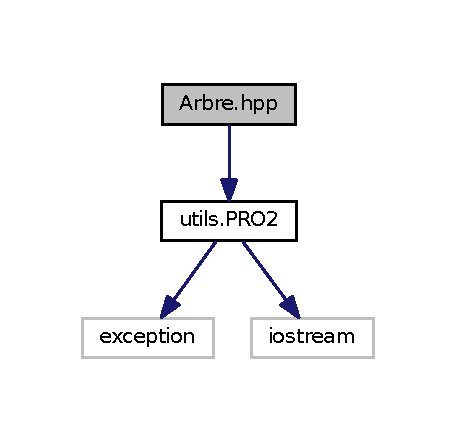
\includegraphics[width=219pt]{_arbre_8hpp__incl}
\end{center}
\end{figure}
\subsection*{Classes}
\begin{DoxyCompactItemize}
\item 
class \hyperlink{class_arbre}{Arbre$<$ T $>$}
\item 
struct \hyperlink{struct_arbre_1_1node__arbre}{Arbre$<$ T $>$\-::node\-\_\-arbre}
\end{DoxyCompactItemize}

\hypertarget{_conjunt_org_8hpp}{\section{Referència del Fitxer Conjunt\-Org.\-hpp}
\label{_conjunt_org_8hpp}\index{Conjunt\-Org.\-hpp@{Conjunt\-Org.\-hpp}}
}


Especificació de la classe \hyperlink{class_conjunt_org}{Conjunt\-Org}.  


Inclou el graf de dependències per a Conjunt\-Org.\-hpp\-:
\nopagebreak
\begin{figure}[H]
\begin{center}
\leavevmode
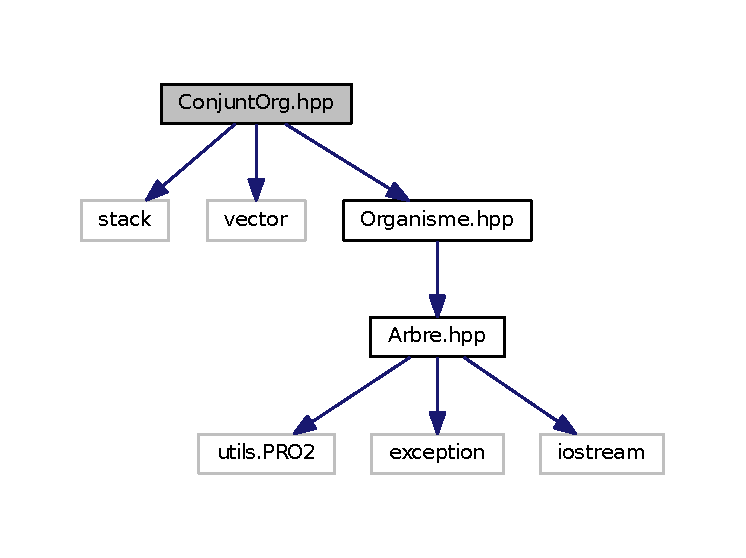
\includegraphics[width=350pt]{_conjunt_org_8hpp__incl}
\end{center}
\end{figure}
\subsection*{Classes}
\begin{DoxyCompactItemize}
\item 
struct \hyperlink{struct_organ_rank}{Organ\-Rank}
\begin{DoxyCompactList}\small\item\em Tipus de dades per poder fer el rànking. \end{DoxyCompactList}\item 
struct \hyperlink{struct_par_fill}{Par\-Fill}
\begin{DoxyCompactList}\small\item\em Estructura per poder saber quins fills ha tingut un organisme i amb qui els ha tingut. \end{DoxyCompactList}\item 
class \hyperlink{class_conjunt_org}{Conjunt\-Org}
\begin{DoxyCompactList}\small\item\em És un conjunt d'organismes. \end{DoxyCompactList}\end{DoxyCompactItemize}


\subsection{Descripció Detallada}
Especificació de la classe \hyperlink{class_conjunt_org}{Conjunt\-Org}. 

Definició al fitxer \hyperlink{_conjunt_org_8hpp_source}{Conjunt\-Org.\-hpp}.


\hypertarget{main_8cpp}{\section{Referència del Fitxer main.\-cpp}
\label{main_8cpp}\index{main.\-cpp@{main.\-cpp}}
}


Programa principal per a la pràctica.  


Inclou el graf de dependències per a main.\-cpp\-:
\nopagebreak
\begin{figure}[H]
\begin{center}
\leavevmode
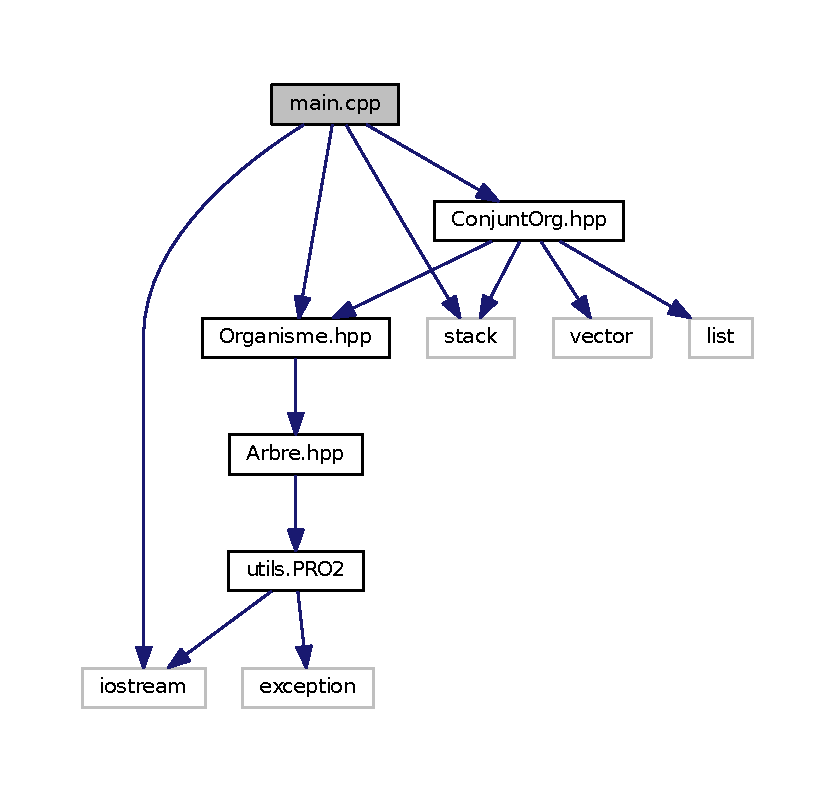
\includegraphics[width=350pt]{main_8cpp__incl}
\end{center}
\end{figure}
\subsection*{Definicions}
\begin{DoxyCompactItemize}
\item 
\#define \hyperlink{main_8cpp_a41985a541fe6a11a9efbe1c57619c004}{M\-A\-R\-C\-A}~-\/1
\end{DoxyCompactItemize}
\subsection*{Funcions}
\begin{DoxyCompactItemize}
\item 
int \hyperlink{main_8cpp_ae66f6b31b5ad750f1fe042a706a4e3d4}{main} ()
\begin{DoxyCompactList}\small\item\em Programa principal de la {\itshape Pràctica de P\-R\-O2}. \end{DoxyCompactList}\end{DoxyCompactItemize}


\subsection{Descripció Detallada}
Programa principal per a la pràctica. 

Definició al fitxer \hyperlink{main_8cpp_source}{main.\-cpp}.



\subsection{Documentació de les Definicions}
\hypertarget{main_8cpp_a41985a541fe6a11a9efbe1c57619c004}{\index{main.\-cpp@{main.\-cpp}!M\-A\-R\-C\-A@{M\-A\-R\-C\-A}}
\index{M\-A\-R\-C\-A@{M\-A\-R\-C\-A}!main.cpp@{main.\-cpp}}
\subsubsection[{M\-A\-R\-C\-A}]{\setlength{\rightskip}{0pt plus 5cm}\#define M\-A\-R\-C\-A~-\/1}}\label{main_8cpp_a41985a541fe6a11a9efbe1c57619c004}


Definició a la línia 18 del fitxer main.\-cpp.



\subsection{Documentació de les Funcions}
\hypertarget{main_8cpp_ae66f6b31b5ad750f1fe042a706a4e3d4}{\index{main.\-cpp@{main.\-cpp}!main@{main}}
\index{main@{main}!main.cpp@{main.\-cpp}}
\subsubsection[{main}]{\setlength{\rightskip}{0pt plus 5cm}int main (
\begin{DoxyParamCaption}
{}
\end{DoxyParamCaption}
)}}\label{main_8cpp_ae66f6b31b5ad750f1fe042a706a4e3d4}


Programa principal de la {\itshape Pràctica de P\-R\-O2}. 



Definició a la línia 22 del fitxer main.\-cpp.


\begin{DoxyCode}
23 \{
24   \textcolor{comment}{// M És el màxim històric permés}
25   \textcolor{comment}{// N És el nombre d'organismes inicials}
26   \textcolor{keywordtype}{int} N, M;
27   cin >> N >> M;
28 
29   \textcolor{comment}{// Conjunt que ens permetrà guardar tots els organismes existents}
30   \hyperlink{class_conjunt_org}{ConjuntOrg} Conj(M);
31     \hyperlink{class_ranking}{Ranking} Rank(M);
32 
33     \textcolor{comment}{// Cridem la funicó per llegir un conjunt d'organismes de la classe}
34     \textcolor{comment}{// ConjuntOrg}
35     Conj.llegir();
36 
37   \textcolor{comment}{// Variable per seleccionar la opció d'entrada}
38   \textcolor{keywordtype}{int} x;
39 
40   \textcolor{comment}{/*  Variable de tipus int que quan sigui diferent de '0' farà}
41 \textcolor{comment}{    acabar l'experiment, un número diferent de 0 indicarà el motiu pel}
42 \textcolor{comment}{    qual s'acaba l'experiment:}
43 \textcolor{comment}{    - 1 => Tots els organismes han mort}
44 \textcolor{comment}{    - 2 => S'ha arribat al límit d'organismes}
45 \textcolor{comment}{    - 3 => S'ha donat per finalitzat l'experiment manualment  */}
46   \textcolor{keywordtype}{int} fi = 0;
47     cin >> x;
48   \textcolor{keywordflow}{while} (x != \hyperlink{main_8cpp_a41985a541fe6a11a9efbe1c57619c004}{MARCA} and fi == 0) \{
49     \textcolor{comment}{// Opció per estirar un conjunt d'organismes}
50         \textcolor{keywordflow}{if} (x == 1) \{
51             \textcolor{keywordtype}{int} a;
52 
53             cin >> a;
54       \textcolor{keywordflow}{while}(a != \hyperlink{main_8cpp_a41985a541fe6a11a9efbe1c57619c004}{MARCA}) \{
55                 Conj.estirar(a);
56         cin >> a;
57             \}
58     \}
59 
60     \textcolor{comment}{// Opció per retallar un conjunt d'organismes}
61         \textcolor{keywordflow}{else} \textcolor{keywordflow}{if} (x == 2) \{
62             \textcolor{keywordtype}{int} a;
63 
64             cin >> a;
65       \textcolor{keywordflow}{while}(a != \hyperlink{main_8cpp_a41985a541fe6a11a9efbe1c57619c004}{MARCA}) \{
66                 Conj.retallar(a);
67         cin >> a;
68             \}
69             \textcolor{keywordflow}{if} (Conj.morts()) fi = 1;
70     \}
71 
72     \textcolor{comment}{// Aplicar una ronda de reproducció a TOTS els organismes, actualitzar}
73     \textcolor{comment}{// el rànking i imprimir els fills nascuts a la ronda}
74     \textcolor{keywordflow}{else} \textcolor{keywordflow}{if} (x == 3) \{
75             \textcolor{keywordtype}{int} fills;
76             \textcolor{keywordflow}{if} (not Conj.reproduir(Rank, fills)) \{
77               fi = 2;
78               x = fills;
79             \}
80             cout << fills << endl;
81     \}
82 
83     \textcolor{comment}{// Obtenir el rànking de reproducció dels organismes }
84     \textcolor{keywordflow}{else} \textcolor{keywordflow}{if} (x == 4) \{
85             Rank.ranking();
86     \}
87 
88     \textcolor{comment}{// Consultar l'estat d'un subconjunt d'organismes }
89         \textcolor{keywordflow}{else} \textcolor{keywordflow}{if} (x == 5) \{
90             \textcolor{keywordtype}{int} a;
91 
92             cin >> a;
93             \textcolor{keywordflow}{while}(a != \hyperlink{main_8cpp_a41985a541fe6a11a9efbe1c57619c004}{MARCA}) \{
94                 Conj.estat(a);
95                 cin >> a;
96             \}
97     \}
98         cin >> x;
99   \}
100 
101     \textcolor{comment}{// Instruccions per a la fi del programa}
102     \textcolor{keywordflow}{if} (fi == 1) \{
103         cout << \textcolor{stringliteral}{"FI: Tots els organismes han mort"} << endl;
104     \}
105     \textcolor{keywordflow}{else} \textcolor{keywordflow}{if} (fi == 2) \{
106         Rank.ranking();
107         Conj.escriure\_ultims(x);
108     \}
109 \}
\end{DoxyCode}

\hypertarget{_organisme_8hpp}{\section{Referència del Fitxer Organisme.\-hpp}
\label{_organisme_8hpp}\index{Organisme.\-hpp@{Organisme.\-hpp}}
}


Especificació de la classe \hyperlink{class_organisme}{Organisme}.  


Inclou el graf de dependències per a Organisme.\-hpp\-:\nopagebreak
\begin{figure}[H]
\begin{center}
\leavevmode
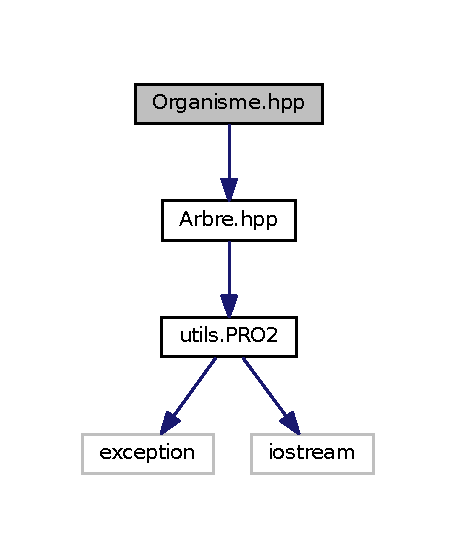
\includegraphics[width=219pt]{_organisme_8hpp__incl}
\end{center}
\end{figure}
\subsection*{Classes}
\begin{DoxyCompactItemize}
\item 
class \hyperlink{class_organisme}{Organisme}
\begin{DoxyCompactList}\small\item\em És un conjunt de cèl·lules posades en un arbre. \end{DoxyCompactList}\item 
struct \hyperlink{struct_organisme_1_1_celula}{Organisme\-::\-Celula}
\begin{DoxyCompactList}\small\item\em Element bàsic de cada organisme. \end{DoxyCompactList}\end{DoxyCompactItemize}


\subsection{Descripció Detallada}
Especificació de la classe \hyperlink{class_organisme}{Organisme}. 

Definició al fitxer \hyperlink{_organisme_8hpp_source}{Organisme.\-hpp}.


\hypertarget{_ranking_8hpp}{\section{Referència del Fitxer Ranking.\-hpp}
\label{_ranking_8hpp}\index{Ranking.\-hpp@{Ranking.\-hpp}}
}


Especificació de la classe \hyperlink{class_ranking}{Ranking}.  


Inclou el graf de dependències per a Ranking.\-hpp\-:\nopagebreak
\begin{figure}[H]
\begin{center}
\leavevmode
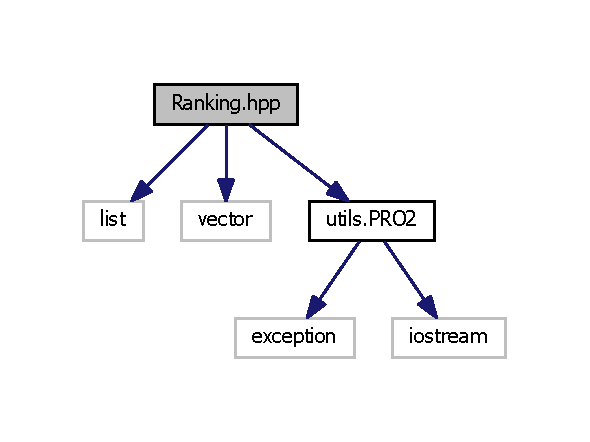
\includegraphics[width=174pt]{_ranking_8hpp__incl}
\end{center}
\end{figure}
\subsection*{Classes}
\begin{DoxyCompactItemize}
\item 
class \hyperlink{class_ranking}{Ranking}
\begin{DoxyCompactList}\small\item\em Classe \hyperlink{class_ranking}{Ranking} per poder imprimir el ranking dels organismes. \end{DoxyCompactList}\item 
struct \hyperlink{struct_ranking_1_1_organ_rank}{Ranking\-::\-Organ\-Rank}
\begin{DoxyCompactList}\small\item\em Estructura que conté l'identificador d'un organisme i el nombre de fills que ha tingut. \end{DoxyCompactList}\item 
struct \hyperlink{struct_ranking_1_1_par_fill}{Ranking\-::\-Par\-Fill}
\begin{DoxyCompactList}\small\item\em Estructura per poder saber quins fills ha tingut un organisme i amb qui els ha tingut. \end{DoxyCompactList}\end{DoxyCompactItemize}


\subsection{Descripció Detallada}
Especificació de la classe \hyperlink{class_ranking}{Ranking}. 

Definició al fitxer \hyperlink{_ranking_8hpp_source}{Ranking.\-hpp}.


\hypertarget{utils_8_p_r_o2}{\section{Referència del Fitxer utils.\-P\-R\-O2}
\label{utils_8_p_r_o2}\index{utils.\-P\-R\-O2@{utils.\-P\-R\-O2}}
}
Inclou el graf de dependències per a utils.\-P\-R\-O2\-:\nopagebreak
\begin{figure}[H]
\begin{center}
\leavevmode
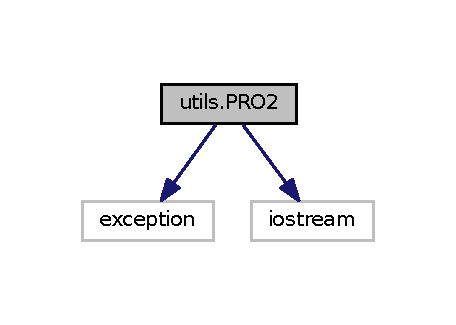
\includegraphics[width=219pt]{utils_8_p_r_o2__incl}
\end{center}
\end{figure}
\subsection*{Classes}
\begin{DoxyCompactItemize}
\item 
class \hyperlink{class_p_r_o2_excepcio}{P\-R\-O2\-Excepcio}
\end{DoxyCompactItemize}
\subsection*{Definicions}
\begin{DoxyCompactItemize}
\item 
\#define \hyperlink{utils_8_p_r_o2_a8610c03aa2297bae1b7872a63c84b353}{U\-T\-I\-L\-S\-\_\-\-P\-R\-O2}
\end{DoxyCompactItemize}
\subsection*{Funcions}
\begin{DoxyCompactItemize}
\item 
int \hyperlink{utils_8_p_r_o2_a49000a716e38017061f71cbefe697a9c}{readint} ()
\item 
char \hyperlink{utils_8_p_r_o2_a831a2329c820ba9b9b378131ed143ff5}{readchar} ()
\item 
bool \hyperlink{utils_8_p_r_o2_a56691e176645da552c107ef124ad701a}{readbool} ()
\item 
double \hyperlink{utils_8_p_r_o2_a2379d4429b4e913e714a3c889061c61c}{readdouble} ()
\item 
string \hyperlink{utils_8_p_r_o2_a0785c313e983db73f256ae0ccf34591c}{readstring} ()
\end{DoxyCompactItemize}


\subsection{Documentació de les Definicions}
\hypertarget{utils_8_p_r_o2_a8610c03aa2297bae1b7872a63c84b353}{\index{utils.\-P\-R\-O2@{utils.\-P\-R\-O2}!U\-T\-I\-L\-S\-\_\-\-P\-R\-O2@{U\-T\-I\-L\-S\-\_\-\-P\-R\-O2}}
\index{U\-T\-I\-L\-S\-\_\-\-P\-R\-O2@{U\-T\-I\-L\-S\-\_\-\-P\-R\-O2}!utils.PRO2@{utils.\-P\-R\-O2}}
\subsubsection[{U\-T\-I\-L\-S\-\_\-\-P\-R\-O2}]{\setlength{\rightskip}{0pt plus 5cm}\#define U\-T\-I\-L\-S\-\_\-\-P\-R\-O2}}\label{utils_8_p_r_o2_a8610c03aa2297bae1b7872a63c84b353}


Definició a la línia 2 del fitxer utils.\-P\-R\-O2.



\subsection{Documentació de les Funcions}
\hypertarget{utils_8_p_r_o2_a49000a716e38017061f71cbefe697a9c}{\index{utils.\-P\-R\-O2@{utils.\-P\-R\-O2}!readint@{readint}}
\index{readint@{readint}!utils.PRO2@{utils.\-P\-R\-O2}}
\subsubsection[{readint}]{\setlength{\rightskip}{0pt plus 5cm}int readint (
\begin{DoxyParamCaption}
{}
\end{DoxyParamCaption}
)}}\label{utils_8_p_r_o2_a49000a716e38017061f71cbefe697a9c}
Funcions per fer lectures de tipus basics. 

Definició a la línia 23 del fitxer utils.\-P\-R\-O2.


\begin{DoxyCode}
24 \{
25   \textcolor{keywordtype}{int} n;
26   cin >> n;
27   \textcolor{keywordflow}{return} n;
28 \}
\end{DoxyCode}
\hypertarget{utils_8_p_r_o2_a831a2329c820ba9b9b378131ed143ff5}{\index{utils.\-P\-R\-O2@{utils.\-P\-R\-O2}!readchar@{readchar}}
\index{readchar@{readchar}!utils.PRO2@{utils.\-P\-R\-O2}}
\subsubsection[{readchar}]{\setlength{\rightskip}{0pt plus 5cm}char readchar (
\begin{DoxyParamCaption}
{}
\end{DoxyParamCaption}
)}}\label{utils_8_p_r_o2_a831a2329c820ba9b9b378131ed143ff5}


Definició a la línia 30 del fitxer utils.\-P\-R\-O2.


\begin{DoxyCode}
31 \{
32   \textcolor{keywordtype}{char} n;
33   cin >> n;
34   \textcolor{keywordflow}{return} n;
35 \}
\end{DoxyCode}
\hypertarget{utils_8_p_r_o2_a56691e176645da552c107ef124ad701a}{\index{utils.\-P\-R\-O2@{utils.\-P\-R\-O2}!readbool@{readbool}}
\index{readbool@{readbool}!utils.PRO2@{utils.\-P\-R\-O2}}
\subsubsection[{readbool}]{\setlength{\rightskip}{0pt plus 5cm}bool readbool (
\begin{DoxyParamCaption}
{}
\end{DoxyParamCaption}
)}}\label{utils_8_p_r_o2_a56691e176645da552c107ef124ad701a}


Definició a la línia 38 del fitxer utils.\-P\-R\-O2.


\begin{DoxyCode}
39 \{
40   \textcolor{keywordtype}{string} n;
41   cin >> n;
42   \textcolor{keywordflow}{if} (n!=\textcolor{stringliteral}{"true"} and n!=\textcolor{stringliteral}{"false"}) \textcolor{keywordflow}{throw} \hyperlink{class_p_r_o2_excepcio}{PRO2Excepcio}(\textcolor{stringliteral}{"S'havia de llegir un boolea"});
43   \textcolor{keywordflow}{return} (n==\textcolor{stringliteral}{"true"});
44 \}
\end{DoxyCode}
\hypertarget{utils_8_p_r_o2_a2379d4429b4e913e714a3c889061c61c}{\index{utils.\-P\-R\-O2@{utils.\-P\-R\-O2}!readdouble@{readdouble}}
\index{readdouble@{readdouble}!utils.PRO2@{utils.\-P\-R\-O2}}
\subsubsection[{readdouble}]{\setlength{\rightskip}{0pt plus 5cm}double readdouble (
\begin{DoxyParamCaption}
{}
\end{DoxyParamCaption}
)}}\label{utils_8_p_r_o2_a2379d4429b4e913e714a3c889061c61c}


Definició a la línia 46 del fitxer utils.\-P\-R\-O2.


\begin{DoxyCode}
47 \{
48   \textcolor{keywordtype}{double} n;
49   cin >> n;
50   \textcolor{keywordflow}{return} n;
51 \}
\end{DoxyCode}
\hypertarget{utils_8_p_r_o2_a0785c313e983db73f256ae0ccf34591c}{\index{utils.\-P\-R\-O2@{utils.\-P\-R\-O2}!readstring@{readstring}}
\index{readstring@{readstring}!utils.PRO2@{utils.\-P\-R\-O2}}
\subsubsection[{readstring}]{\setlength{\rightskip}{0pt plus 5cm}string readstring (
\begin{DoxyParamCaption}
{}
\end{DoxyParamCaption}
)}}\label{utils_8_p_r_o2_a0785c313e983db73f256ae0ccf34591c}


Definició a la línia 53 del fitxer utils.\-P\-R\-O2.


\begin{DoxyCode}
54 \{
55   \textcolor{keywordtype}{string} s;
56   cin >> s;
57   \textcolor{keywordflow}{return} s;
58 \}
\end{DoxyCode}

\addcontentsline{toc}{part}{Índex}
\printindex
\end{document}
